\documentclass{report}
\usepackage{tocloft}
\usepackage{amsmath}
\usepackage{color,pxfonts,fix-cm}
\usepackage{latexsym}
\usepackage[mathletters]{ucs}
\usepackage[T1]{fontenc}
\usepackage[utf8x]{inputenc}
\usepackage{pict2e}
\usepackage{wasysym}
\usepackage[english]{babel}
\usepackage{tikz}
\usepackage[margin=1in]{geometry}
\usepackage{amsmath}
\usepackage{array}
\setcounter{tocdepth}{2}
\usepackage{graphicx}
\usepackage{caption}
\usepackage{ragged2e}
\usepackage{mathrsfs}
\usepackage{float}
\usepackage{parskip}
\geometry{a4paper}
\usepackage{multirow}
\usepackage{fancyhdr}
\usepackage{url}
\usepackage{comment}

% Page style
\pagestyle{empty}
\pagestyle{fancy}
\fancyfoot[C]{\thepage}
\renewcommand{\headrulewidth}{0pt}
\renewcommand{\cftchapleader}{\cftdotfill{\cftdotsep}}
\renewcommand{\cftsecleader}{\cftdotfill{\cftdotsep}}
\renewcommand{\cftsubsecleader}{\cftdotfill{\cftdotsep}}
\begin{document}

% Title
\begin{center}
    \textbf{\Large HUMAN AWARE RE-IDENTIFICATION AND TRACKING}\\[20pt]
    \textbf{\Large A Project Progress Report}\\[20pt]
    Submitted in partial fulfillment for the degree of\\[20pt]
    \textbf{\Large BACHELOR OF TECHNOLOGY}\\[20pt]
    in\\[20pt]
    \textbf{\Large COMPUTER SCIENCE AND ENGINEERING}\\[20pt]
    Submitted by\\[20pt]
   \begin{center}
    \begin{tabbing}
    \centering
       \hspace{2cm} K.HARSHITHA \hspace{7cm} \= (N200373) \\\hspace{2cm}
        CH.RAJESWARI\> (N200427) \\\hspace{2cm}
        B.CHETHAN \> (N200518) \\\hspace{2cm}
        SK.AKHIL\> (N200145) \\\hspace{2cm}
    \end{tabbing}
    \end{center}

    Under the Esteem Guidance of\\[10pt]
    \textbf{Y.KALAVATHI}\\[40pt]
    \includegraphics[width=1in]{rguktlogo.png}\\[40pt]
    \textbf{\Large DEPARTMENT OF COMPUTER SCIENCE AND ENGINEERING}\\[10pt]
    \textbf{ Rajiv Gandhi University of Knowledge Technologies -- Nuzvid}\\[10pt]
    \textbf{ Nuzvid, Eluru, Andhra Pradesh -- 521202}
\end{center}

% Certificate
\newpage
\begin{center}
    \includegraphics[width=1in]{rguktlogo.png}\\[40pt]
    \textbf{\Large DEPARTMENT OF COMPUTER SCIENCE AND ENGINEERING}\\[10pt]
    \textbf{Rajiv Gandhi University of Knowledge Technologies -- Nuzvid}\\[10pt]
    \textbf{Nuzvid, Eluru, Andhra Pradesh -- 521202}
\end{center}

\vspace{30pt} % Adds vertical space between sections

\begin{center}
    \textbf{\Large \underline{CERTIFICATE OF COMPLETION}}\\[30pt]
\end{center}

\noindent
\normalsize{This is to certify that the work entitled, \textbf{``HUMAN AWARE RE-IDENTIFICATION AND TRACKING''} is the bonafide work of \textbf{K.HARSHITHA (N200373), CH.RAJESWARI (N200427),\vspace{3pt} B.CHETHAN (N200518), SK.AKHIL (N200145)} carried out under my guid\vspace{3pt}ance and supervision for 4th year project of Bachelor of Technology in the department of Computer\vspace{3pt} Science and Engineering under RGUKT IIIT Nuzvid. This work is done during the academic session\vspace{3pt} August 2025 -- April 2026, under our guidance.}\\[60pt]

\begin{tabbing}
    \hspace{3in} \= \hspace{1.5in} \= \kill
    ---------------------------------------- \> \> ------------------------------------- \\
    Y.Kalavathi\> \> A.Uday Kumar  \\
    Mentor, \> \> Assistant Professor, \\
    Department of CSE, \> \> Head of the Department, \\
    RGUKT Nuzvid. \> \> Department of CSE, \\
    \> \> RGUKT Nuzvid.
\end{tabbing}

\newpage

\setlength{\parindent}{0pt}
\setlength{\parskip}{1em}

\begin{center}
\includegraphics[width=1in]{rguktlogo.png}\\[40pt]
    \textbf{\Large DEPARTMENT OF COMPUTER SCIENCE AND ENGINEERING}\\[10pt]
    \textbf{ Rajiv Gandhi University of Knowledge Technologies -- Nuzvid}\\[10pt]
    \textbf{ Nuzvid, Eluru, Andhra Pradesh -- 521202}\\
\end{center}
\vspace{30pt}
\begin{center}
    \textbf{\Large \underline{CERTIFICATE OF EXAMINATION}}\\[30pt]
\end{center}
\normalsize{This is to certify that the work entitled,\textbf{``HUMAN AWARE RE-IDENTIFICATION AND TRACKING''} is the bonafied work of \textbf{K.HARSHITHA (N200373), CH.RAJESWARI (N200427),\vspace{3pt} B.CHETHAN (N200518), SK.AKHIL (N200145)} and here by accord our approval of it as a study carried out and presented in a manner re\vspace{3pt}quired for its acceptance in 4th year of \textbf{Bachelor of Technology} for which it has been submitted. This\vspace{3pt} approval does not necessarily endorse or accept every statement made, opinion expressed or conclusion\vspace{3pt} drawn, as a recorded in this thesis. It only signifies the acceptance of this thesis for the purpose for\vspace{3pt} which it has been submitted.}\\[50pt]
\large{
    \begin{tabbing}
    \hspace{3in} \= \hspace{1.6in} \= \kill
    ------------------------------------------- \> \> ------------------------------ \\
   Y.Kalavathi \> \> Project Examiner \\
    Mentor, \> \> RGUKT-Nuzvid \\
    Department of CSE, \> \> \\
    RGUKT-NUZVID \> \>
    \end{tabbing}
    }

\newpage
\begin{center}
\includegraphics[width=1 in]{rguktlogo.png}\\[40pt]
    \textbf{\Large DEPARTMENT OF COMPUTER SCIENCE AND ENGINEERING}\\[10pt]
    \textbf{Rajiv Gandhi University of Knowledge Technologies -- Nuzvid}\\[10pt]
    \textbf{Nuzvid, Eluru, Andhra Pradesh -- 521202}\\
\end{center}
\vspace{30pt}
\begin{center}
    \textbf{\Large \underline{DECLARATION}}\\[30pt]
\end{center}

\noindent
\normalsize{We, \textbf{K.HARSHITHA (N200373), CH.RAJESWARI (N200427),\vspace{3pt} B.CHETHAN (N200518), SK.AKHIL (N200145)} hereby declare that the project report entitled \textbf{``HUMAN AWARE RE-IDENTIFICATION AND TRACKING''} done by us under the guidance of Y.Kalavathi, is submitted\vspace{3pt} for the partial fulfillment of the award of degree of Bachelor of Technology in Computer Science and\vspace{3pt} Engineering during the academic session August 2025 - April 2026 at RGUKT-Nuzvid.

We also declare that this project is a result of our own effort and has not been copied or imitated from\vspace{3pt} any source. Citations from any websites are mentioned in the references. The results embodied in this\vspace{3pt} project report have not been submitted to any other university or institute for the award of any degree\vspace{3pt} or diploma.}

\vspace{0.2in}
    \noindent
    \large

\begin{tabbing}
Date: 29-04-2025 \hspace{1.6in} \= B.KOMALI SRAVYA \hspace{0.5in} \= (N190163) \kill
Date: 10-04-2026 \>K.HARSHITHA \> (N200373) \\
Place: Nuzvid \> CH.RAJESWARI \> (N200427) \\
\> B.CHETHAN \> (N200518) \\
\> SK.AKHIL \> (N200145) \\
\end{tabbing}
    \vspace{0.2in}

% ─── ACKNOWLEDGEMENT ──────────────────────────────────────────────────────────
\newpage

\begin{center}
    \textbf{\Large {ACKNOWLEDGEMENT}}\\[20pt]
\end{center}

\noindent
\normalsize{We would like to express our profound gratitude and deep regards to our guide \textbf{Y.Kalavathi}\vspace{3pt} for his exemplary guidance, monitoring, and constant encouragement throughout the B.Tech course.\vspace{3pt} We shall always cherish the time spent with him during the course of this work due to the invaluable\vspace{3pt} knowledge gained in the field of reliability engineering.

We are extremely grateful for the confidence bestowed upon us and for entrusting us with our project\vspace{3pt} entitled \textbf{``HUMAN AWARE RE-IDENTIFICATION AND TRACKING''}.

We express our gratitude to \textbf{Mr.A.Uday Kumar} (HOD of CSE) and other faculty members for\vspace{3pt} being a source of inspiration and constant encouragement, which helped us in completing the project\vspace{3pt} successfully.

Our sincere thanks go to all the batchmates of 2020 CSE, who have made our stay at RGUKT-NUZVID\vspace{3pt} a memorable one.

Finally, yet importantly, we would like to express our heartfelt thanks to our beloved God and parents\vspace{3pt} for their blessings, and our friends for their help and wishes for the successful completion of this project.}

% ─── CHAPTER 1: ABSTRACT ──────────────────────────────────────────────────────
\newpage
\begin{center}
    \section*{\textbf{CHAPTER 1}}
\end{center}
\begin{center}
    \textbf{\Large ABSTRACT}\\[20pt]
\end{center}

\noindent
\normalsize{Human tracking and biometric identification have become essential components in modern intelligent\vspace{3pt} surveillance and attendance management systems. With increasing reliance on automated systems in\vspace{3pt} academic and institutional environments, there is a strong need for solutions that can accurately detect,\vspace{3pt} track, and identify individuals in real-time from live video streams or pre-recorded footage, even under\vspace{3pt} conditions of occlusion, re-entry, pose variation, and lighting change.

This project presents a real-time biometric attendance management system that integrates computer\vspace{3pt} vision, deep learning, and a web-based interface to fully automate student attendance in classroom\vspace{3pt} environments. The system combines multi-object person detection, persistent tracking, and face recogni\vspace{3pt}tion into a unified pipeline capable of processing both live webcam feeds and uploaded MP4 recordings\vspace{3pt} through a single platform.

Person detection is performed using YOLOv11n, a lightweight single-stage detector, and each detected\vspace{3pt} individual is assigned a persistent identity across frames using the BoT-SORT multi-object tracker with\vspace{3pt} Kalman filter-based motion prediction. Face recognition is handled by InsightFace (Buffalo\_L model),\vspace{3pt} which extracts 512-dimensional facial embeddings for identity matching via cosine similarity. A two-tier\vspace{3pt} matching strategy is employed: a dynamic session cache storing up to five diverse embeddings per student\vspace{3pt} enables fast in-session recognition, while a persistent per-section database serves as the fallback for\vspace{3pt} new detections.

Recognition reliability is ensured through a consensus-based locking mechanism that requires agree\vspace{3pt}ment across multiple frames before confirming an identity, reducing false positives from single-frame\vspace{3pt} noise. Adaptive shadow updates continuously refine session embeddings in the background to account\vspace{3pt} for changes in lighting and pose over the course of a session. Unknown individuals who cannot be\vspace{3pt} matched are detected, logged with captured snapshots, and tracked separately as visitors.

Attendance is recorded using a heartbeat-based interval logging mechanism that fires every ten seconds,\vspace{3pt} synchronising the database and maintaining continuous entry and exit timestamps for each student. This\vspace{3pt} enables computation of precise attendance durations, detection of mid-session absences, and generation\vspace{3pt} of per-student time-in-room analytics. The system is backed by a Django web dashboard providing live\vspace{3pt} MJPEG video streaming, real-time attendance monitoring, session controls, and a reports interface with\vspace{3pt} CSV export.

The system incorporates an SLM Orchestration pipeline that emits structured telemetry events throughout\vspace{3pt} each session and, on session completion, queries a locally hosted small language model (Ollama\vspace{3pt} Qwen2.5:1.5b) to generate a human-readable session narrative report without any dependency on\vspace{3pt} external APIs or cloud services.

Overall, the proposed system provides a scalable, robust, and accurate solution for automated attendance\vspace{3pt} management, combining the reliability of deep learning-based face recognition with the transparency of\vspace{3pt} structured analytics and AI-generated reporting to reduce manual effort and improve institutional insight\vspace{3pt} generation.}

% ─── TABLE OF CONTENTS ────────────────────────────────────────────────────────
\newpage
\begin{center}
    \textbf{\Large Table of Contents}
\end{center}
\addcontentsline{toc}{chapter}{Table of Contents}
\noindent
\begin{tabbing}
    \hspace{1cm} \= \hspace{11cm} \= \hspace{2cm} \= \kill
    \textbf{CHAPTER 1 \> \> \> 6} \\[0.2cm]
    \textbf{ABSTRACT \> \> \> 6} \\[0.2cm]
    \\
    \textbf{CHAPTER 2 \> \> \> 9--14} \\[0.2cm]
    \textbf{INTRODUCTION \> \> \> 9--14} \\[0.2cm]
    2.1 \> Motivation for the Work \> \> 9--10 \\[0.2cm]
    \hspace{1cm} \= \hspace{11cm} \= \hspace{2cm} \= \kill
    2.2 \> Real-world Applications \> \> 10--11 \\[0.2cm]
    2.3 \> Problem Statement \> \> 12--14 \\[0.2cm]
    \\
    \textbf{CHAPTER 3 \> \> \> 15--21} \\[0.2cm]
    \textbf{RELATED WORKS \> \> \> 15--21} \\[0.2cm]
    3.1 \> Background on Object Detection \> \> 15--16 \\[0.2cm]
    3.2 \> Background on Multi-Object Tracking \> \> 16--17 \\[0.2cm]
    3.3 \> Background on Face Recognition \> \> 17--18 \\[0.2cm]
    3.4 \> Existing Attendance Systems \> \> 18--20 \\[0.2cm]
    3.5 \> Small Language Models for Analytics \> \> 20--21 \\[0.2cm]
    \\
    \textbf{CHAPTER 4 \> \> \> 22--38} \\[0.2cm]
    \textbf{PROPOSED METHOD \> \> \> 22--38} \\[0.2cm]
    4.1 \> System Overview \> \> 22 \\[0.2cm]
    4.2 \> System Flowchart \> \> 23 \\[0.2cm]
    4.3 \> System Architecture \> \> 24 \\[0.2cm]
    4.4 \> Components in the Flowchart \> \> 25--33 \\[0.2cm]
    \> 4.4.1 Student Registration \> \> 25 \\[0.2cm]
    \> 4.4.2 Session Initialization \> \> 25--26 \\[0.2cm]
    \> 4.4.3 Video Input \> \> 26 \\[0.2cm]
    \> 4.4.4 Person Detection and Tracking \> \> 26--27 \\[0.2cm]
    \> 4.4.5 Face Recognition \> \> 27--28 \\[0.2cm]
    \> 4.4.6 Identity Consensus Check \> \> 28--29 \\[0.2cm]
    \> 4.4.7 Attendance Marking \> \> 29--30 \\[0.2cm]
    \> 4.4.8 Interval Tracking \> \> 30--31 \\[0.2cm]
    \> 4.4.9 Session End and Report Generation \> \> 31--33 \\[0.2cm]
    4.5 \> Algorithms \> \> 34--38 \\[0.2cm]
    \> 4.5.1 Algorithm for Recognition and Consensus \> \> 34--36 \\[0.2cm]
    \> 4.5.2 Algorithm for Heartbeat Interval Tracking \> \> 36--38 \\[0.2cm]
    \\
    \textbf{CHAPTER 5 \> \> \> 39--50} \\[0.2cm]
    \textbf{EXPERIMENTAL RESULTS \> \> \> 39--50} \\[0.2cm]
    5.1 \> Technologies and Libraries Used \> \> 39--40 \\[0.2cm]
    5.2 \> Dataset and Enrollment \> \> 40--41 \\[0.2cm]
    5.3 \> System Requirements \> \> 41 \\[0.2cm]
    5.4 \> Results \> \> 42--47 \\[0.2cm]
    \> 5.4.1 Live Dashboard \> \> 42 \\[0.2cm]
    \> 5.4.2 Session Report Page \> \> 43 \\[0.2cm]
    \> 5.4.3 MP4 Batch Processing \> \> 44 \\[0.2cm]
    \> 5.4.4 AI-Generated Session Report \> \> 45 \\[0.2cm]
    \> 5.4.5 Recognition Performance Metrics \> \> 46--47 \\[0.2cm]
    5.5 \> Comparison with Existing Approaches \> \> 48--50 \\[0.2cm]
    \\
    \textbf{CHAPTER 6 \> \> \> 51} \\[0.2cm]
    \textbf{CONCLUSION \> \> \> 51} \\[0.2cm]
    \\
    \textbf{CHAPTER 7 \> \> \> 52} \\[0.2cm]
    \textbf{FUTURE SCOPE \> \> \> 52} \\[0.2cm]
    \\
    \textbf{CHAPTER 8 \> \> \> 53} \\[0.2cm]
    \textbf{REFERENCES \> \> \> 53} \\[0.2cm]
\end{tabbing}

% ─── CHAPTER 2: INTRODUCTION ──────────────────────────────────────────────────
\newpage
\begin{center}
    \section*{\textbf{CHAPTER 2}}
\end{center}
\begin{center}
    \textbf{\Large INTRODUCTION}\\[20pt]
\end{center}

\subsection*{2.1 Motivation for the Work}
In today's digital era, large volumes of video data are generated continuously through surveillance\vspace{3pt} cameras in institutions, organizations, and public spaces. However, manually monitoring and analyzing\vspace{3pt} this data is time-consuming, inefficient, and prone to human error.

Traditional attendance systems, such as manual roll calls, RFID-based methods, or simple fingerprint\vspace{3pt} scanners, suffer from several critical limitations. Proxy attendance remains a persistent problem, as\vspace{3pt} one student can sign on behalf of another without being detected. Such systems also provide no insight\vspace{3pt} into actual presence duration: a student who enters and immediately leaves is recorded as fully present.\vspace{3pt} Furthermore, they offer no real-time monitoring capability, making it impossible for faculty to know\vspace{3pt} the current state of the classroom at any given moment.

With the rapid advancement of deep learning and computer vision, modern techniques such as object\vspace{3pt} detection, multi-object tracking, and face recognition provide an opportunity to build intelligent,\vspace{3pt} automated systems that fundamentally overcome these limitations. By treating every student as an\vspace{3pt} object to be continuously detected and identified across video frames, it becomes possible to measure\vspace{3pt} not just whether a student attended but how long they were physically present.

The motivation behind this project is to develop a robust, real-time biometric attendance system that:

\begin{itemize}
    \item Accurately detects and tracks multiple students simultaneously from a single camera
    \item Maintains consistent identities across frames even through occlusions and re-entries
    \item Records precise entry and exit timestamps for each student
    \item Detects and logs unknown individuals who are not enrolled in the system
    \item Provides a web-based interface for live monitoring, control, and session reporting
    \item Generates AI-driven narrative reports summarizing each session automatically
\end{itemize}

This system aims to eliminate proxy attendance, provide verifiable time-in-room records, and give\vspace{3pt} faculty a complete, intelligent view of classroom attendance with minimal manual effort.

\subsection*{2.2 Real-world Applications}
The proposed system has a wide range of applications across different domains where real-time human\vspace{3pt} identification and presence tracking are essential.

\begin{enumerate}

\item \textbf{Smart Classroom Attendance}
\begin{itemize}
    \item Automatically records student attendance using face recognition from a single camera
    \item Captures entry and exit timestamps for accurate duration tracking
    \item Eliminates proxy attendance and reduces faculty workload
\end{itemize}

\item \textbf{Workplace and Employee Monitoring}
\begin{itemize}
    \item Tracks employee attendance and precise working hours
    \item Identifies authorized and unauthorized personnel in restricted areas
    \item Can be integrated with HR management systems
\end{itemize}

\item \textbf{Surveillance and Security}
\begin{itemize}
    \item Detects and tracks individuals in real-time video streams
    \item Flags unknown or unregistered persons with snapshot capture
    \item Applicable in campuses, airports, and public areas
\end{itemize}

\item \textbf{Batch Video Processing}
\begin{itemize}
    \item Processes pre-recorded MP4 lecture videos for retrospective attendance
    \item Useful when live monitoring infrastructure is not available
    \item Produces the same structured reports as live sessions
\end{itemize}

\item \textbf{Healthcare and Laboratory Access}
\begin{itemize}
    \item Tracks movement of students, staff, or patients in restricted zones
    \item Maintains entry/exit logs for compliance and safety purposes
\end{itemize}

\item \textbf{Exam Hall Monitoring}
\begin{itemize}
    \item Verifies student presence throughout the examination duration
    \item Detects and logs persons who enter or exit during the exam
    \item Provides timestamped records for audit purposes
\end{itemize}

\item \textbf{Smart Campus Infrastructure}
\begin{itemize}
    \item Integrates with existing campus network and databases
    \item Supports multi-section, multi-session deployment
    \item Generates structured analytics for institutional reporting
\end{itemize}

\end{enumerate}

\subsection*{2.3 Problem Statement}
Despite the availability of face recognition and computer vision technologies, existing automated\vspace{3pt} attendance solutions remain largely inadequate for real-world academic deployment. The key problems\vspace{3pt} that motivated this project are described below.

\textbf{Proxy Attendance:} Traditional biometric systems such as fingerprint scanners only verify attendance\vspace{3pt} at a single point in time. They cannot detect whether a student leaves the classroom immediately\vspace{3pt} after being marked, enabling partial attendance to be recorded as full attendance.

\textbf{Identity Instability in Video:} Simple face recognition systems applied to video suffer from\vspace{3pt} identity switching, where the same individual may be assigned different identities across frames\vspace{3pt} due to pose changes, occlusion, or lighting variation. Without a multi-frame consensus mechanism,\vspace{3pt} this leads to unreliable attendance records.

\textbf{Absence of Duration Tracking:} Most existing systems record binary present/absent states without\vspace{3pt} capturing how long each student was actually present. This prevents meaningful analytics such as\vspace{3pt} bunk detection, late arrival identification, and early departure logging.

\textbf{Lack of Real-Time Visibility:} Faculty typically receive attendance data only after a session\vspace{3pt} ends. There is no live view of who is currently present, making real-time intervention impossible.

\textbf{No Unknown Person Detection:} Conventional systems only verify enrolled individuals. They\vspace{3pt} cannot detect or log the presence of unknown visitors, security risks, or non-enrolled persons.

\textbf{Single-Mode Operation:} Most systems operate only in live mode. There is no provision for\vspace{3pt} processing pre-recorded videos, which is critical for retrospective attendance or when a camera\vspace{3pt} was set up but not monitored in real time.

\textbf{No AI-Driven Reporting:} Existing systems produce raw attendance tables. There is no mechanism\vspace{3pt} to generate human-readable summaries of system behavior, recognition quality, or attendance\vspace{3pt} patterns for faculty review.

The proposed system directly addresses each of these limitations through a combination of multi-object\vspace{3pt} tracking, consensus-based face recognition, heartbeat-driven interval logging, a live web dashboard,\vspace{3pt} and an integrated small language model reporting pipeline.

% ─── CHAPTER 3: RELATED WORKS ─────────────────────────────────────────────────
\newpage
\begin{center}
    \section*{\textbf{CHAPTER 3}}
\end{center}
\begin{center}
    \textbf{\Large RELATED WORKS}\\[20pt]
\end{center}

\subsection*{3.1 Background on Object Detection}

Object detection is a fundamental computer vision task that involves both classifying what is present\vspace{3pt} in an image and localizing where each object is. Historically, detection relied on handcrafted features\vspace{3pt} such as Histogram of Oriented Gradients (HOG) combined with Support Vector Machine (SVM) classi\vspace{3pt}fiers, or Haar-like features with AdaBoost. While effective under controlled conditions, these methods\vspace{3pt} degrade significantly with changes in scale, lighting, and pose.

The deep learning era introduced two-stage detectors such as R-CNN, Fast R-CNN, and Faster R-CNN,\vspace{3pt} which first generate region proposals and then classify each region. These models achieve high accuracy\vspace{3pt} but suffer from slow inference, making them unsuitable for real-time applications.

Single-stage detectors eliminated the region proposal step by predicting bounding boxes and class\vspace{3pt} probabilities directly from the input image. YOLO (You Only Look Once) was a landmark contribution\vspace{3pt} in this space, enabling real-time detection in a single forward pass. Successive versions, from YOLOv2\vspace{3pt} through YOLOv11, have progressively improved accuracy, speed, and robustness through improved\vspace{3pt} backbone architectures, feature pyramid networks, and advanced anchor-free detection heads.

In this project, \textbf{YOLOv11n} (the nano variant of YOLOv11) is used as the person detector. It offers\vspace{3pt} an excellent balance of speed and accuracy, detecting persons in real time at approximately 30 frames\vspace{3pt} per second on consumer hardware. Only detections of class 0 (person) are retained, and confidence\vspace{3pt} thresholds are tuned based on camera region: 0.30 for the front zone and 0.15 for the rear of the\vspace{3pt} classroom, where individuals are smaller and less clearly visible.

\subsection*{3.2 Background on Multi-Object Tracking}

Multi-Object Tracking (MOT) is the task of associating detected objects across video frames to maintain\vspace{3pt} consistent identities over time. The tracking-by-detection paradigm uses a separate detector in each\vspace{3pt} frame and links the resulting bounding boxes using motion and appearance cues.

The Kalman Filter is a widely used probabilistic estimator that predicts an object's future position\vspace{3pt} based on its past trajectory and a motion model. When a new detection arrives, the tracker compares\vspace{3pt} it with predicted states to determine whether it belongs to an existing track or represents a new object.

SORT (Simple Online and Realtime Tracking) combines Kalman filtering for state prediction with\vspace{3pt} Intersection-over-Union (IoU) matching for data association. While computationally efficient, SORT\vspace{3pt} frequently loses identity during brief occlusions. DeepSORT addresses this by incorporating appearance\vspace{3pt} embeddings from a deep neural network to improve association in crowded scenes. StrongSORT further\vspace{3pt} enhances this with camera motion compensation and exponential moving average feature smoothing.

\textbf{BoT-SORT} (Bootstrap Object Tracking using SORT) is the tracker selected for this system. It extends\vspace{3pt} SORT with global motion compensation via sparse optical flow, improving robustness against camera\vspace{3pt} movement. In this project, the built-in Re-ID module of BoT-SORT is disabled in favor of a custom\vspace{3pt} multi-vector InsightFace-based Re-ID layer, providing higher accuracy for face-based identity matching\vspace{3pt} than generic appearance features.

\subsection*{3.3 Background on Face Recognition}

Face recognition systems typically operate in three stages: face detection, feature extraction, and\vspace{3pt} identity matching. Modern deep learning-based systems extract compact, discriminative embeddings\vspace{3pt} from face images that represent identity in a high-dimensional space. Similarity between two embeddings\vspace{3pt} is measured using cosine or Euclidean distance, with a threshold.

\textbf{InsightFace} is a widely adopted open-source framework that provides state-of-the-art face analysis\vspace{3pt} models. The Buffalo\_L model used in this project generates 512-dimensional face embeddings using\vspace{3pt} an ArcFace-trained backbone, which optimizes for maximum inter-class separation and intra-class\vspace{3pt} compactness. This makes it robust to small variations in pose and lighting, which is essential for\vspace{3pt} classroom deployment where students are not required to look directly at the camera.

Cosine similarity between embeddings is computed as:
\begin{equation}
    \text{similarity}(a, b) = \frac{a \cdot b}{\|a\| \cdot \|b\|}
\end{equation}
A score above the threshold confirms identity. In this system, a threshold of 0.45 is used for\vspace{3pt} database lookup and 0.50 for session cache matching.

\subsection*{3.4 Existing Attendance Systems}

Early automated attendance systems used RFID cards or fingerprint biometrics, reducing manual effort\vspace{3pt} but introducing proxy opportunities and binary presence recording. Vision-based systems using\vspace{3pt} simple frame-by-frame face recognition improved accuracy but lacked tracking continuity, leading to\vspace{3pt} identity switching under real classroom conditions.

Recent works have integrated detection, tracking, and recognition pipelines. However, most existing\vspace{3pt} systems share common limitations:

\begin{itemize}
    \item No stateful interval tracking: they record a final present/absent state rather than continuous\vspace{3pt} entry and exit windows
    \item No multi-frame consensus: single-frame recognition leads to false positives
    \item No unknown person handling: unregistered individuals are silently ignored
    \item No real-time web interface: systems operate as standalone scripts without live monitoring
    \item No support for batch video processing alongside live sessions
    \item No AI-generated reporting: output is limited to raw attendance tables
\end{itemize}

The proposed system addresses all of the above limitations with a unified, production-grade\vspace{3pt} architecture.

\subsection*{3.5 Small Language Models for Analytics}


Small Language Models (SLMs) are compact, locally deployable models that retain useful language\vspace{3pt} generation ability while running entirely on-device. Recent SLMs such as the Qwen2.5 series offer\vspace{3pt} models as small as 1.5 billion parameters that can run on CPU-only hardware without requiring a GPU.

In this project, \textbf{Ollama Qwen2.5:1.5b} is used post-session to generate a structured Markdown report\vspace{3pt} from the session's telemetry log. Since the model runs locally via the Ollama runtime, no student\vspace{3pt} data leaves the institution's network, addressing both latency and privacy requirements. This represents\vspace{3pt} a novel application of SLMs in the context of automated attendance reporting.

% ─── CHAPTER 4: PROPOSED METHOD ───────────────────────────────────────────────
\newpage
\begin{center}
    \section*{\textbf{CHAPTER 4}}
\end{center}
\begin{center}
    \textbf{\Large PROPOSED METHOD}\\[20pt]
\end{center}

\subsection*{4.1 System Overview}
The proposed system is a multi-layered real-time biometric attendance pipeline built around a\vspace{3pt} separation of concerns between the computer vision engine and the web interface. The core recognition\vspace{3pt} engine (\texttt{main.py}) runs as an independent subprocess, handling all camera I/O, detection, tracking,\vspace{3pt} and database writes. The Django web layer acts as an operator interface, sending control commands\vspace{3pt} via file-based inter-process communication (IPC) and reading results from the shared SQLite database\vspace{3pt} and MJPEG frame files.

The system supports two input modes: live webcam sessions for real-time classroom attendance, and\vspace{3pt} MP4 upload sessions for processing pre-recorded lecture videos. Both modes produce identical structured\vspace{3pt} output in the database and generate the same report types. A global process lock ensures that only\vspace{3pt} one session (webcam or MP4) can run at a time, preventing resource conflicts.

Student enrollment is a one-time offline step performed using \texttt{register\_student.py}, which captures\vspace{3pt} face images and stores a 512-D InsightFace embedding per student in a section-specific pickle file.\vspace{3pt} These embeddings serve as the ground truth for all subsequent recognition.

\subsection*{4.2 System Flowchart}

Figure \ref{fig:flowchart} presents the complete high-level process flow of the system, from session\vspace{3pt} initialization through face recognition, attendance marking, interval tracking, and final report generation.

\begin{figure}[htbp]
    \centering
    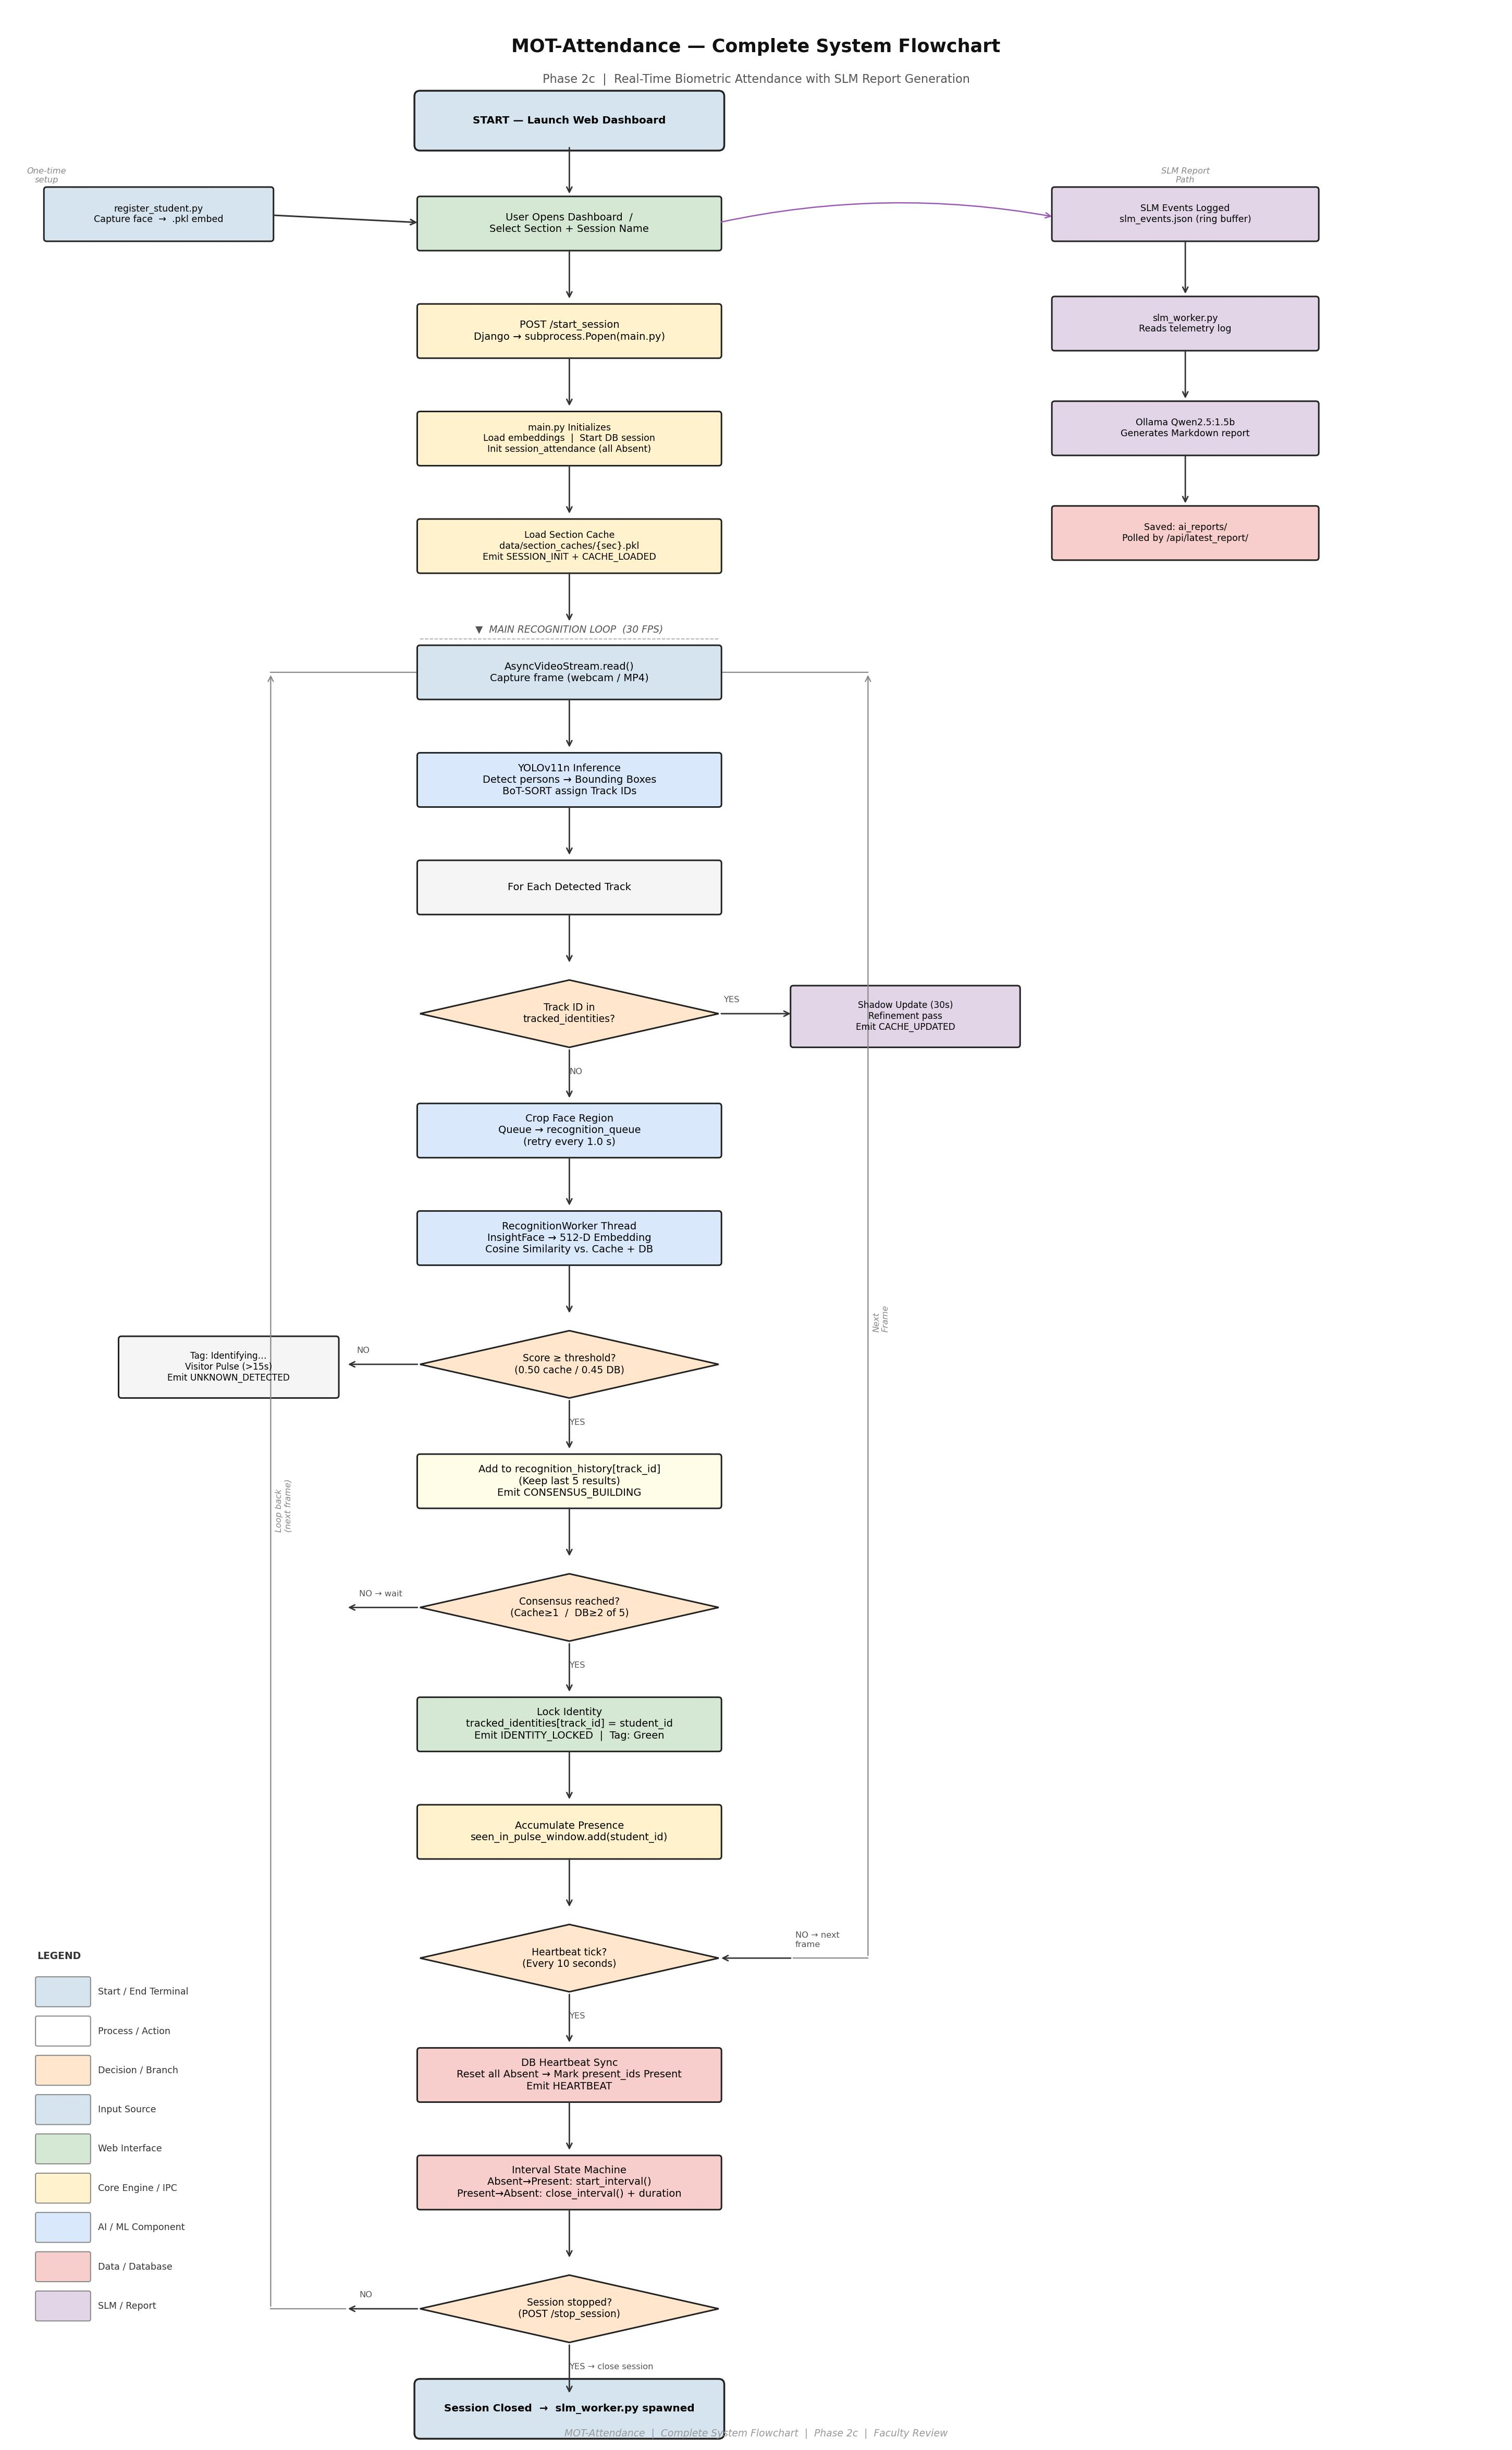
\includegraphics[width=0.62\textwidth]{assets/Flowchart_Final.jpg}
    \caption{High-Level System Flowchart for Real-Time Biometric Attendance}
    \label{fig:flowchart}
\end{figure}

\subsection*{4.3 System Architecture}

Figure \ref{fig:architecture} presents the layered system architecture, illustrating the relationship\vspace{3pt} between the input sources, web interface, core engine, AI/ML pipeline, SLM orchestration layer,\vspace{3pt} and the data layer.

\begin{figure}[htbp]
    \centering
    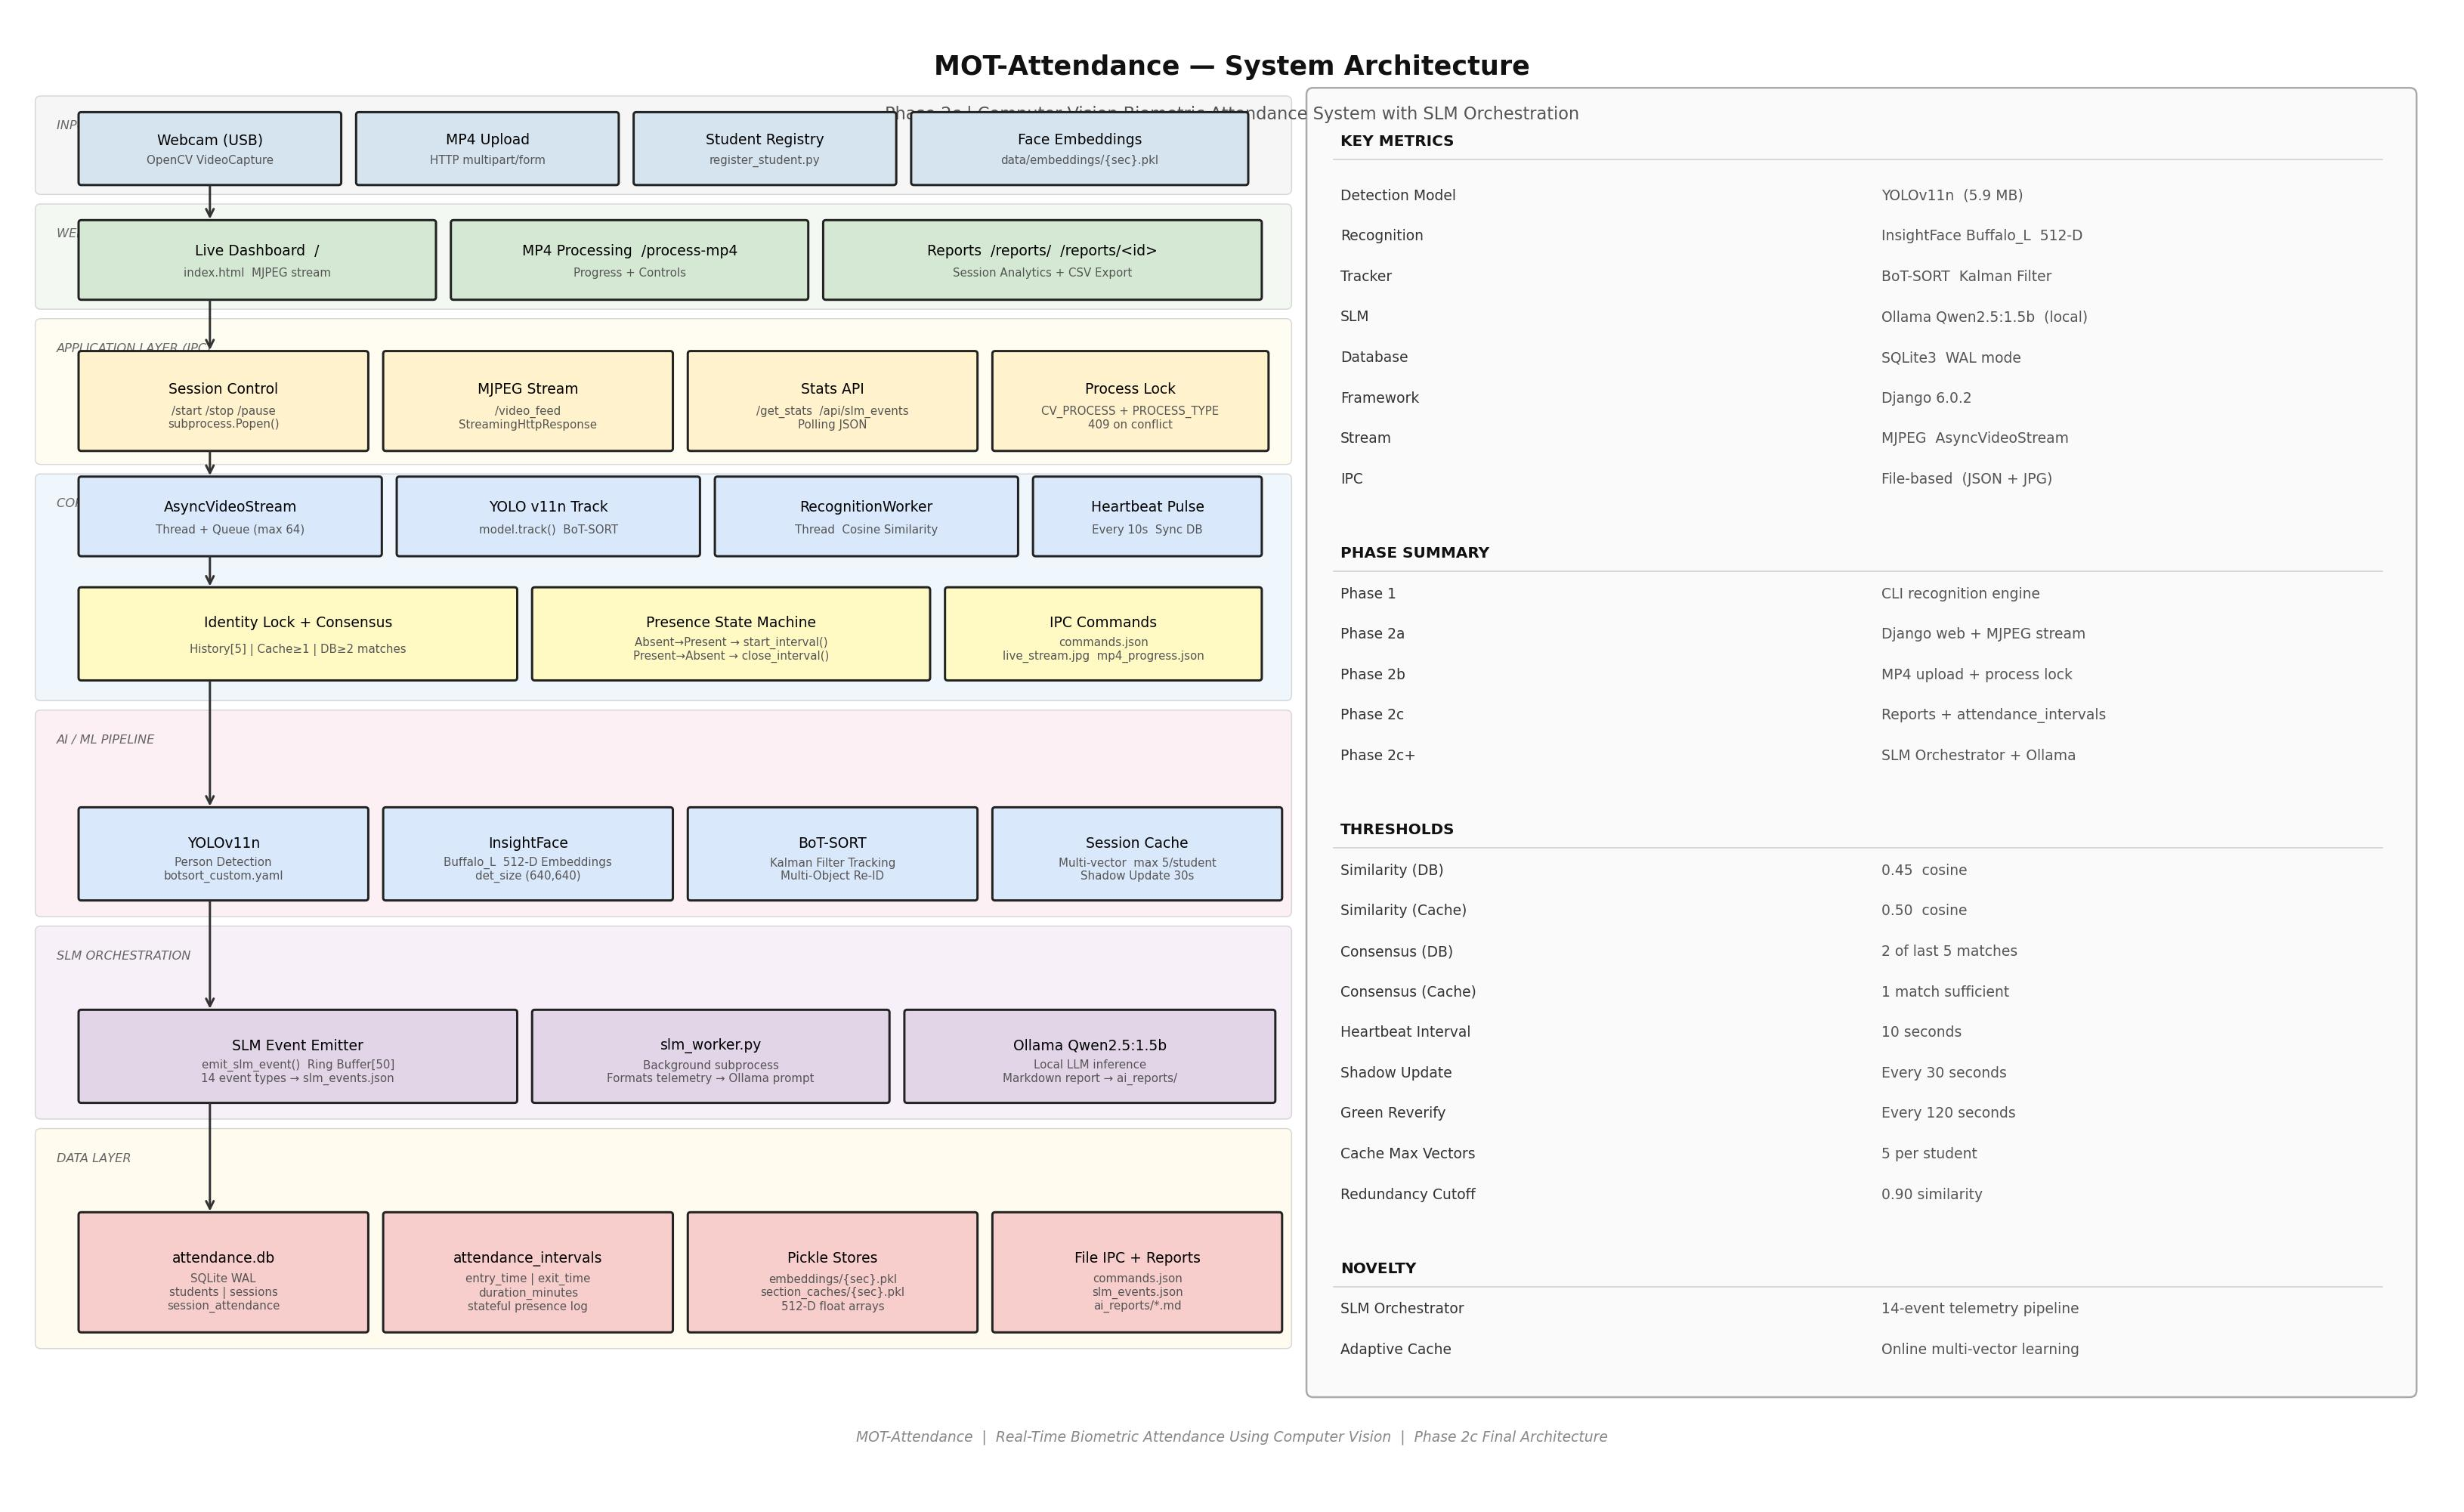
\includegraphics[width=\textwidth]{assets/Architecture_Final.jpg}
    \caption{Layered System Architecture -- Phase 2c}
    \label{fig:architecture}
\end{figure}

The architecture is organized into seven layers. The \textbf{Input Layer} provides video from either\vspace{3pt} a connected webcam or an uploaded MP4 file, alongside the student face embedding files and the\vspace{3pt} student registry. The \textbf{Web Interface Layer} provides three browser-accessible pages: the live\vspace{3pt} dashboard, the MP4 processing page, and the reports interface. The \textbf{Application Layer} handles\vspace{3pt} HTTP routing, session lifecycle management, MJPEG streaming, and inter-process communication.\vspace{3pt} The \textbf{Core Engine Layer} runs entirely within \texttt{main.py} as a subprocess and contains the main\vspace{3pt} recognition loop, identity locking logic, and presence state machine. The \textbf{AI/ML Layer} provides\vspace{3pt} YOLOv11n detection, InsightFace embedding extraction, BoT-SORT tracking, and the adaptive session\vspace{3pt} cache. The \textbf{SLM Orchestration Layer} emits structured telemetry events throughout the session\vspace{3pt} and invokes Ollama post-session for report generation. The \textbf{Data Layer} stores all structured records\vspace{3pt} in SQLite and face embeddings in pickle files.

\subsection*{4.4 Components in the Flowchart}

\subsubsection*{4.4.1 Student Registration (One-Time Setup)}
\normalsize{
Before any attendance session can be conducted, each student must be enrolled into the system using\vspace{3pt} the \texttt{register\_student.py} command-line utility. During registration, the student faces the camera\vspace{3pt} and multiple frame captures are taken. The InsightFace Buffalo\_L model processes each captured frame\vspace{3pt} to extract a 512-dimensional face embedding, which serves as the student's biometric identity template.

The student's name, roll number, and section are stored in the \texttt{students} table of the SQLite\vspace{3pt} database, and the embedding is appended to the section-specific pickle file at\vspace{3pt} \texttt{data/embeddings/\{section\}.pkl}. This one-time process needs to be performed only once per\vspace{3pt} student, and the resulting embeddings persist across all future sessions for that section. The quality\vspace{3pt} of the enrollment capture directly influences recognition accuracy during live sessions.
}

\subsubsection*{4.4.2 Session Initialization}
\normalsize{
A faculty operator opens the web dashboard at \texttt{http://127.0.0.1:8000} and clicks Start Session.\vspace{3pt} A modal dialog allows selection of the academic section (auto-populated by scanning available\vspace{3pt} embedding files) and entry of a session name. Upon confirmation, the Django view issues a\vspace{3pt} \texttt{subprocess.Popen()} call that launches \texttt{main.py} with the selected section and session name\vspace{3pt} as arguments.

The recognition engine then initializes by: (1) loading all student embeddings for the selected\vspace{3pt} section from the pickle store, (2) pre-loading the section-specific session cache if one exists from\vspace{3pt} a prior session, (3) creating a new row in the \texttt{sessions} table, (4) inserting a row for every\vspace{3pt} student in the section into \texttt{session\_attendance} with status set to Absent, and (5) emitting\vspace{3pt} \texttt{SESSION\_INIT} and \texttt{CACHE\_LOADED} events to the SLM telemetry log. A 19-second countdown\vspace{3pt} loader on the dashboard provides visual feedback during model initialization.
}

\subsubsection*{4.4.3 Video Input}
\normalsize{
The system supports two video input modes. In \textbf{live webcam mode}, frames are read from the\vspace{3pt} connected USB camera using OpenCV's \texttt{VideoCapture(0)}, wrapped in a dedicated\vspace{3pt} \texttt{AsyncVideoStream} thread that reads frames into a bounded queue of maximum size 64. This\vspace{3pt} prevents the recognition pipeline from blocking camera I/O, ensuring a consistent 30 FPS capture\vspace{3pt} rate regardless of downstream processing speed.

In \textbf{MP4 batch mode}, the operator uploads a pre-recorded video through the browser. The file is\vspace{3pt} saved to \texttt{data/uploads/} and the same \texttt{AsyncVideoStream} reads from the file path instead\vspace{3pt} of a camera index. Frame stride is set to 2x for MP4 processing to accelerate throughput, since\vspace{3pt} consecutive frames in a recording contain minimal new information. Both modes write processed\vspace{3pt} (annotated) frames to \texttt{data/live\_stream.jpg} for MJPEG streaming to the browser.
}

\subsubsection*{4.4.4 Person Detection and Tracking}
\normalsize{
Each captured frame is passed to the YOLOv11n model with persistent BoT-SORT tracking enabled.\vspace{3pt} The model outputs bounding boxes, class labels, confidence scores, and track IDs for all detected\vspace{3pt} objects. Only detections of class 0 (person) are retained. A confidence threshold of 0.30 is applied\vspace{3pt} to the front 65\% of the frame, where individuals are larger and more clearly visible, while a lower\vspace{3pt} threshold of 0.15 is applied to the rear zone to capture students seated further from the camera.

BoT-SORT maintains a Kalman filter state for each tracked person, predicting their position in the\vspace{3pt} next frame using a linear motion model. The Hungarian algorithm is used to solve the track-detection\vspace{3pt} assignment problem each frame. Each person receives a unique integer track ID that persists as long\vspace{3pt} as the tracker maintains continuity, even through brief occlusions or missed detections. This track\vspace{3pt} ID becomes the key used by all subsequent recognition and attendance logic.
}

\subsubsection*{4.4.5 Face Recognition}
\normalsize{
For each active track, the system crops the face region from the bounding box and passes it to the\vspace{3pt} InsightFace recognition worker, which runs on a dedicated background thread to avoid blocking the\vspace{3pt} main detection loop. The worker calls \texttt{app.get(crop)} to extract a 512-D embedding from the\vspace{3pt} cropped face image.

This embedding is then compared against two sources. First, the \textbf{session cache} is queried:\vspace{3pt} a dictionary of up to five diverse embeddings per student, built from confirmed recognitions during\vspace{3pt} the current and previous sessions. Cosine similarity is computed against each cached vector, and a\vspace{3pt} match is declared if any score exceeds 0.50. If the session cache yields no match, the \textbf{full database\vspace{3pt} embeddings} for the section are searched with a lower threshold of 0.45.

Only faces meeting a minimum quality threshold (detection score above 0.6 and face size above\vspace{3pt} 60$\times$60 pixels) are submitted for recognition. Low-quality crops are skipped to prevent noise from\vspace{3pt} degrading the recognition history.
}

\subsubsection*{4.4.6 Identity Consensus Check}
\normalsize{
A single successful recognition match is not immediately accepted as a confirmed identity. Instead,\vspace{3pt} the match result is appended to a rolling recognition history buffer of length 5 per track ID. This\vspace{3pt} history is used to compute a consensus decision, preventing false positives that may arise from a\vspace{3pt} single noisy frame.

The consensus threshold depends on the match source. A cache hit requires only \textbf{1 match} in\vspace{3pt} the history to confirm identity, since session cache vectors correspond to previously verified poses.\vspace{3pt} A database match, coming from a static enrollment embedding, requires \textbf{2 matches out of the last\vspace{3pt} 5 frames} before identity is confirmed. Once consensus is reached, the track is locked: a mapping\vspace{3pt} from track ID to student ID is stored in \texttt{tracked\_identities} and the student's bounding box is\vspace{3pt} annotated with a green label and their name. The system emits an \texttt{IDENTITY\_LOCKED} event to\vspace{3pt} the SLM telemetry log at this point.

If no consensus is reached after 15 seconds, the track is classified as an unknown visitor. Its\vspace{3pt} bounding box is annotated in gray, a snapshot is saved to \texttt{data/unknown\_faces/}, and an\vspace{3pt} \texttt{UNKNOWN\_DETECTED} event is emitted. The visitor pulse mechanism re-attempts recognition every\vspace{3pt} 12 seconds in case the student's face becomes more clearly visible later.
}

\subsubsection*{4.4.7 Attendance Marking}
\normalsize{
Recognized student IDs are accumulated in a set called \texttt{seen\_in\_pulse\_window} throughout each\vspace{3pt} 10-second window. At the end of every window, a \textbf{heartbeat pulse} fires. This pulse performs a\vspace{3pt} single atomic database operation: it resets all rows in \texttt{session\_attendance} for the current session\vspace{3pt} to Absent, then marks all student IDs in \texttt{seen\_in\_pulse\_window} as Present. The window is then\vspace{3pt} cleared for the next 10-second cycle.

This heartbeat design provides robustness against momentary occlusions. A student who is briefly\vspace{3pt} blocked from view for one or two frames within a 10-second window is still counted as present for\vspace{3pt} that window. Only a sustained absence of a full 10 seconds results in the student being marked Absent.\vspace{3pt} The live dashboard polls the database every 2 seconds and updates the attendance table and present\vspace{3pt} count in real time, giving faculty immediate visibility into who is currently in the classroom.

Additionally, the adaptive \textbf{shadow update} mechanism runs every 30 seconds for each recognized\vspace{3pt} student. A silent re-recognition pass is performed on their current face crop, and if the resulting\vspace{3pt} embedding is sufficiently different from existing cache entries (cosine similarity below 0.90), it is\vspace{3pt} added to the session cache. This allows the system to progressively learn new poses and lighting\vspace{3pt} conditions throughout the session, improving recognition accuracy over time.
}

\subsubsection*{4.4.8 Interval Tracking}
\normalsize{
The 10-second heartbeat pulse also drives a \textbf{presence state machine} for each student. Each student\vspace{3pt} has an associated state: \texttt{is\_present} (boolean) and \texttt{active\_interval\_id} (integer or null). These\vspace{3pt} states determine transitions in the \texttt{attendance\_intervals} table.

When a student transitions from Absent to Present (i.e., they appear in \texttt{seen\_in\_pulse\_window}\vspace{3pt} after not appearing in the previous window), \texttt{db.start\_interval()} is called. This inserts a new\vspace{3pt} row into \texttt{attendance\_intervals} with \texttt{entry\_time} set to the current timestamp, \texttt{exit\_time}\vspace{3pt} as NULL, and sets \texttt{is\_present = True}.

When a student transitions from Present to Absent (absent from the current window after being\vspace{3pt} present), \texttt{db.close\_interval()} is called. This updates the open row with \texttt{exit\_time = now()} and\vspace{3pt} computes \texttt{duration\_minutes = (exit\_time - entry\_time) / 60}. A student who enters, leaves, and\vspace{3pt} re-enters will produce two or more distinct interval rows, each with its own entry, exit, and duration.\vspace{3pt} The session report page aggregates these intervals to compute total time present and to detect\vspace{3pt} bunk windows (gaps between consecutive intervals).
}

\subsubsection*{4.4.9 Session End and Report Generation}
\normalsize{
When the faculty clicks Stop Session, the Django view writes \texttt{\{"stop": true\}} to\vspace{3pt} \texttt{data/commands.json}. The recognition engine polls this file every few frames and, upon detecting\vspace{3pt} the stop command, performs a graceful shutdown: it closes all open presence intervals, sets the session\vspace{3pt} status to CLOSED in the database, exports the updated session cache to\vspace{3pt} \texttt{data/section\_caches/\{section\}.pkl} for use in future sessions, and emits a\vspace{3pt} \texttt{SESSION\_CLOSED} event.

Immediately after shutdown, \texttt{main.py} spawns \texttt{slm\_worker.py} as a background subprocess.\vspace{3pt} This worker reads the full telemetry log from \texttt{data/slm\_events.json}, formats it as a structured\vspace{3pt} text prompt, and sends it to the locally running Ollama Qwen2.5:1.5b model. The model generates\vspace{3pt} a Markdown-formatted session narrative report covering attendance summary, recognition quality\vspace{3pt} observations, and system learning events. The report is saved to\vspace{3pt} \texttt{data/ai\_reports/ai\_report\_\{session\}\_\{timestamp\}.md}.

On the web dashboard, the Report Drawer polls \texttt{/api/latest\_report/} and renders the AI report\vspace{3pt} using the \texttt{marked.js} Markdown library. The faculty can also navigate to \texttt{/reports/} to view all\vspace{3pt} sessions, and to \texttt{/reports/\{session\_id\}/} for the full per-student interval breakdown, total durations,\vspace{3pt} bunk intervals, and the option to download a CSV export.
}

\subsection*{4.5 Algorithms}

\subsubsection*{4.5.1 Algorithm for Real-Time Face Recognition and Identity Consensus}

\subsection*{Step 1: Start}
Initialize the recognition engine. Load section embeddings from \texttt{data/embeddings/\{section\}.pkl}\vspace{3pt} into the database embedding store. Load the persistent section cache from\vspace{3pt} \texttt{data/section\_caches/\{section\}.pkl} if available. Initialize all state dictionaries:\vspace{3pt} \texttt{tracked\_identities}, \texttt{recognition\_history}, \texttt{session\_cache}, \texttt{last\_verified\_time}.

\subsection*{Step 2: Capture Frame}
Read the next frame from \texttt{AsyncVideoStream}. If the queue is empty, wait. Retrieve the\vspace{3pt} (frame\_index, frame) tuple. Apply frame stride (skip alternate frames for MP4 mode).

\subsection*{Step 3: Detect and Track Persons}
Pass the frame to the YOLOv11n model with \texttt{persist=True} and BoT-SORT tracker. Filter\vspace{3pt} results to class 0 (person) only. Apply regional confidence thresholds. Extract the list of\vspace{3pt} (bounding\_box, track\_id, confidence) tuples.

\subsection*{Step 4: For Each Detected Track}
Crop the face region from the bounding box. Check whether the \texttt{track\_id} already exists in\vspace{3pt} \texttt{tracked\_identities}.

\begin{itemize}
    \item \textbf{If unknown (not in \texttt{tracked\_identities}):} check if the retry cooldown (1.0 s) has elapsed\vspace{3pt} since last recognition attempt. If yes, enqueue the face crop to \texttt{recognition\_queue}.
    \item \textbf{If known:} check if the shadow update interval (30 s) has elapsed. If yes, silently enqueue\vspace{3pt} the crop for adaptive cache refinement.
    \item \textbf{If known and re-verify interval (120 s) has elapsed:} enqueue for full reverification.
\end{itemize}

\subsection*{Step 5: Recognition Worker (Background Thread)}
Dequeue (track\_id, crop) from \texttt{recognition\_queue}. Extract 512-D embedding via InsightFace.\vspace{3pt} Validate face quality: detection score $>$ 0.6 and size $>$ 60$\times$60 pixels. If quality fails, discard.

Compute cosine similarity against session cache embeddings:
\begin{equation}
    s_i = \frac{e \cdot c_i}{\|e\| \cdot \|c_i\|}
\end{equation}
where $e$ is the query embedding and $c_i$ is the $i$-th cached embedding. If $\max(s_i) \geq 0.50$, record a cache hit for the corresponding student. Otherwise, compute similarity against all database embeddings and check against threshold 0.45.

\subsection*{Step 6: Build Consensus}
Append the best matching student ID (or ``unknown'') to \texttt{recognition\_history[track\_id]}.\vspace{3pt} Maintain only the last 5 entries. Count occurrences of each student ID in the history.

\begin{itemize}
    \item If the count of the best student $\geq$ 1 (cache hit) or $\geq$ 2 (DB hit): declare identity locked.
    \item Set \texttt{tracked\_identities[track\_id] = student\_id}.
    \item Emit \texttt{IDENTITY\_LOCKED} event. Update session cache with the current embedding.
    \item If count $<$ threshold: emit \texttt{CONSENSUS\_BUILDING} (once per track).
\end{itemize}

\subsection*{Step 7: Adaptive Cache Update}
After identity lock, if the new embedding is sufficiently diverse (similarity to all existing cache\vspace{3pt} entries below 0.90), append it to the session cache. If cache size exceeds 5, replace the most\vspace{3pt} similar existing entry. Emit \texttt{CACHE\_UPDATED} or \texttt{CACHE\_SKIPPED} accordingly.

\subsection*{Step 8: Accumulate Presence}
Add the locked student ID to \texttt{seen\_in\_pulse\_window}.

\subsection*{Step 9: Heartbeat Check}
If 10 seconds have elapsed since the last heartbeat, trigger the heartbeat pulse (see Algorithm 4.5.2).\vspace{3pt} Reset \texttt{seen\_in\_pulse\_window}.

\subsection*{Step 10: Repeat or Terminate}
Return to Step 2. If \texttt{data/commands.json} contains \texttt{\{"stop": true\}}: proceed to Step 11.

\subsection*{Step 11: End}
Close all open intervals. Update session status to CLOSED. Save section cache to disk.\vspace{3pt} Spawn \texttt{slm\_worker.py} as a background subprocess. Terminate.

\subsubsection*{4.5.2 Algorithm for Heartbeat-Based Attendance Interval Tracking}

\subsection*{Step 1: Start}
Initialize \texttt{seen\_in\_pulse\_window = \{\}} and \texttt{student\_presence\_state = \{\}} for all\vspace{3pt} enrolled students in the section. Each entry in \texttt{student\_presence\_state} holds\vspace{3pt} \texttt{is\_present = False} and \texttt{active\_interval\_id = None}.

\subsection*{Step 2: Accumulate Window}
During the current 10-second window, for every recognized student ID, add it to\vspace{3pt} \texttt{seen\_in\_pulse\_window}. This step runs continuously in the background as the main recognition\vspace{3pt} loop processes frames.

\subsection*{Step 3: Heartbeat Trigger (Every 10 Seconds)}
Call \texttt{db.global\_heartbeat\_sync(session\_id, present\_ids)} where\vspace{3pt} \texttt{present\_ids = seen\_in\_pulse\_window}. This operation atomically resets all rows in\vspace{3pt} \texttt{session\_attendance} for the current session to Absent, then marks all IDs in \texttt{present\_ids}\vspace{3pt} as Present.

\subsection*{Step 4: For Each Student in present\_ids (Present Transition)}
Retrieve \texttt{state = student\_presence\_state[student\_id]}.\\
If \texttt{state.is\_present == False}:
\begin{itemize}
    \item Call \texttt{db.start\_interval(session\_id, student\_id)} $\rightarrow$ inserts row with\vspace{3pt} \texttt{entry\_time = now()}, \texttt{exit\_time = NULL}.
    \item Store returned interval ID in \texttt{state.active\_interval\_id}.
    \item Set \texttt{state.is\_present = True}.
    \item Emit \texttt{INTERVAL\_START} event with student name and timestamp.
\end{itemize}

\subsection*{Step 5: For Each Student NOT in present\_ids (Absent Transition)}
Retrieve \texttt{state = student\_presence\_state[student\_id]}.\\
If \texttt{state.is\_present == True}:
\begin{itemize}
    \item Call \texttt{db.close\_interval(state.active\_interval\_id)}:
    \begin{itemize}
        \item Updates row: \texttt{exit\_time = now()}
        \item Computes: \texttt{duration\_minutes = (exit\_time - entry\_time).total\_seconds() / 60}
    \end{itemize}
    \item Set \texttt{state.is\_present = False}, \texttt{state.active\_interval\_id = None}.
    \item Emit \texttt{INTERVAL\_END} event with student name, duration.
\end{itemize}

\subsection*{Step 6: Emit Heartbeat Event}
Emit \texttt{HEARTBEAT} event with current present count. Reset \texttt{seen\_in\_pulse\_window = \{\}}.

\subsection*{Step 7: Repeat Until Session End}
Return to Step 2. Continue until \texttt{commands.json} signals stop.

\subsection*{Step 8: End}
On session end, call \texttt{db.close\_interval()} for all students with \texttt{is\_present == True}\vspace{3pt} to ensure no open intervals remain. All interval records are now available for the reports page.

% ─── CHAPTER 5: EXPERIMENTAL RESULTS ─────────────────────────────────────────
\newpage
\begin{center}
    \section*{\textbf{CHAPTER 5}}
\end{center}
\begin{center}
    \textbf{\Large EXPERIMENTAL RESULTS}\\[20pt]
\end{center}

\subsection*{5.1 Technologies and Libraries Used}

\begin{itemize}
\normalsize{
    \item \textbf{Python 3.12}: The primary programming language used for the entire system. Python's\vspace{3pt} ecosystem of computer vision and machine learning libraries, combined with its threading and\vspace{3pt} subprocess support, made it the natural choice for this project.

    \item \textbf{Ultralytics YOLOv11}: Used for real-time person detection. The nano variant (YOLOv11n)\vspace{3pt} provides the best speed-accuracy trade-off for single-camera classroom deployment, running\vspace{3pt} inference at approximately 30 FPS on consumer CPU hardware.

    \item \textbf{InsightFace (Buffalo\_L)}: The core face recognition framework. Provides ArcFace-trained\vspace{3pt} 512-dimensional embeddings with support for CoreML acceleration on Apple Silicon and CPU\vspace{3pt} inference on all platforms.

    \item \textbf{OpenCV (cv2)}: Used for video capture, frame preprocessing, face region cropping,\vspace{3pt} JPEG encoding of live stream frames, and video writing for session exports.

    \item \textbf{Django 6.0.2}: The web framework powering the dashboard. Provides template rendering,\vspace{3pt} HTTP routing, and \texttt{StreamingHttpResponse} for MJPEG video delivery.

    \item \textbf{SQLite3}: The embedded relational database storing all students, sessions, attendance\vspace{3pt} records, and interval data. Configured in WAL (Write-Ahead Logging) mode for concurrent\vspace{3pt} access between the recognition engine and web layer.

    \item \textbf{Ollama (Qwen2.5:1.5b)}: A locally hosted small language model runtime used for\vspace{3pt} post-session AI report generation. Requires no internet connection and processes the\vspace{3pt} telemetry log entirely on-device.

    \item \textbf{NumPy}: Used for embedding storage, cosine similarity computation, and array\vspace{3pt} operations within the recognition pipeline.

    \item \textbf{Pickle}: Used for serializing and deserializing 512-D face embedding arrays for\vspace{3pt} per-section storage and session cache persistence.

    \item \textbf{marked.js}: A JavaScript Markdown-to-HTML library used in the browser to render\vspace{3pt} the AI-generated session report within the Report Drawer panel.
}
\end{itemize}

\subsection*{5.2 Dataset and Enrollment}
Unlike benchmark datasets with fixed labeled images, this system uses a live enrollment model where\vspace{3pt} the dataset is built per-section through \texttt{register\_student.py}. Each student faces the camera\vspace{3pt} from multiple angles and a 512-D InsightFace embedding is stored in the section pickle file. The\vspace{3pt} system was evaluated with \textbf{34 students} enrolled in section \textbf{CSE\_1}, with enrollment\vspace{3pt} taking approximately 2--3 minutes per student. Over the academic period, \textbf{126 sessions} were\vspace{3pt} conducted. The adaptive session cache progressively refined embeddings across sessions, improving\vspace{3pt} recognition speed for returning students in subsequent classes.

\subsection*{5.3 System Requirements}

\textbf{Hardware:}
\begin{itemize}
    \item \textbf{Processor}: 64-bit multi-core CPU, 2.6 GHz or higher
    \item \textbf{RAM}: 8 GB minimum; 16 GB recommended for smooth MP4 processing
    \item \textbf{Camera}: USB webcam (720p or higher)
    \item \textbf{Storage}: 2 GB minimum for model weights, embeddings, and session data
\end{itemize}

\textbf{Software:}
\begin{itemize}
    \item Python 3.12+, pip dependencies from \texttt{requirements.txt}
    \item Ollama runtime with \texttt{qwen2.5:1.5b} model pulled locally
    \item Django 6.0.2 development server or production WSGI server
    \item macOS / Linux / Windows 64-bit
\end{itemize}

\subsection*{5.4 Results}

The system was evaluated across four operational modes.

\noindent\textbf{5.4.1~--~Live Dashboard:} the root route (\texttt{/}) streams live MJPEG video with
bounding-box overlays; the attendance table refreshes every 2\,s and a statistics panel shows
present count, enrolled total, and unknown-detection alerts.

\noindent\textbf{5.4.2~--~Session Report:} the page at \texttt{/reports/\{session\_id\}/} lists
per-student entry/exit timestamps, total duration, bunk intervals, and offers a CSV export.

\noindent\textbf{5.4.3~--~MP4 Batch Processing:} \texttt{/process-mp4} accepts uploaded lecture videos
and runs the full recognition pipeline retrospectively with a live progress bar and
pause/resume controls.

\noindent\textbf{5.4.4~--~AI Report:} after each session the SLM worker calls Ollama Qwen2.5:1.5b
locally to produce a Markdown narrative covering attendance summary, recognition quality,
adaptive-cache events, and timeline highlights (late arrivals, early departures).

Screenshots of all four system views are shown on the following two pages.

% ════════════════════════════════════════════════════════════════════════════
%  SCREENSHOT PAGE 1 — Dashboard  +  Session Report
% ════════════════════════════════════════════════════════════════════════════
\newpage
\begin{figure}[H]
    \centering
    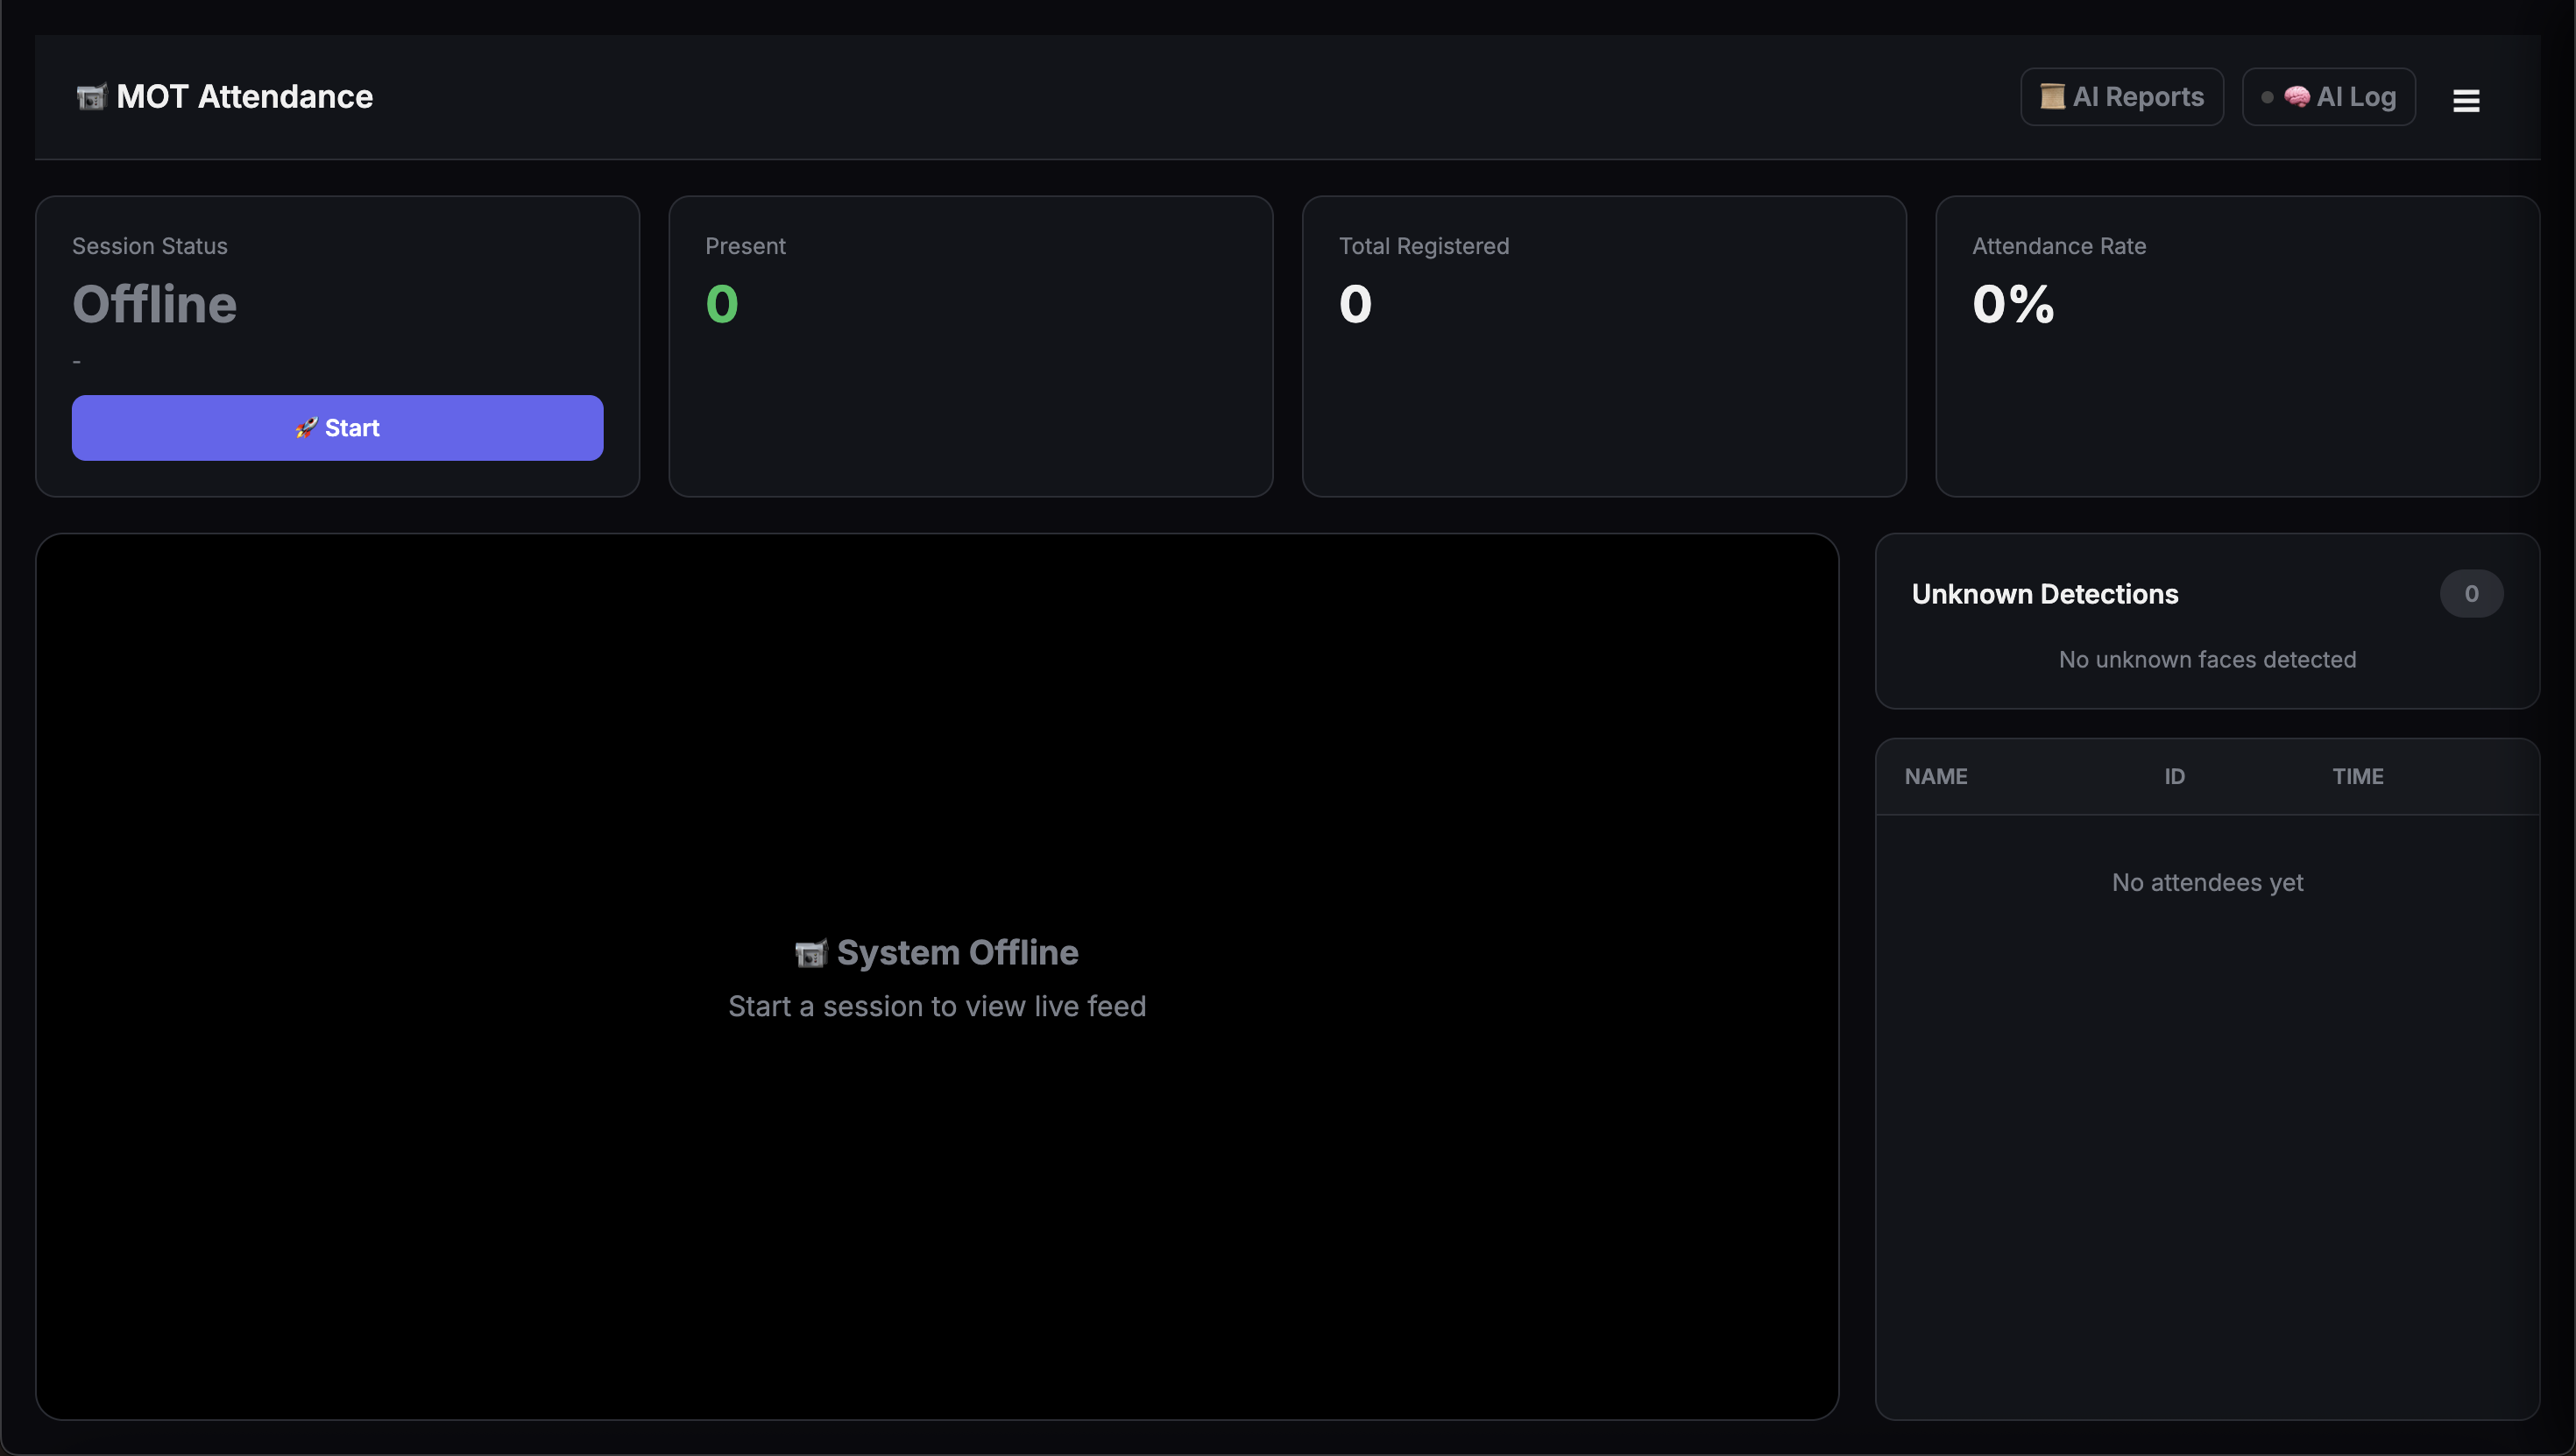
\includegraphics[width=\textwidth, height=0.43\textheight, keepaspectratio]{screenshot_dashboard.png}
    \caption{5.4.1 \ Live Dashboard -- Real-Time Attendance Monitoring}
    \label{fig:dashboard}
\end{figure}

\vspace{6pt}

\begin{figure}[H]
    \centering
    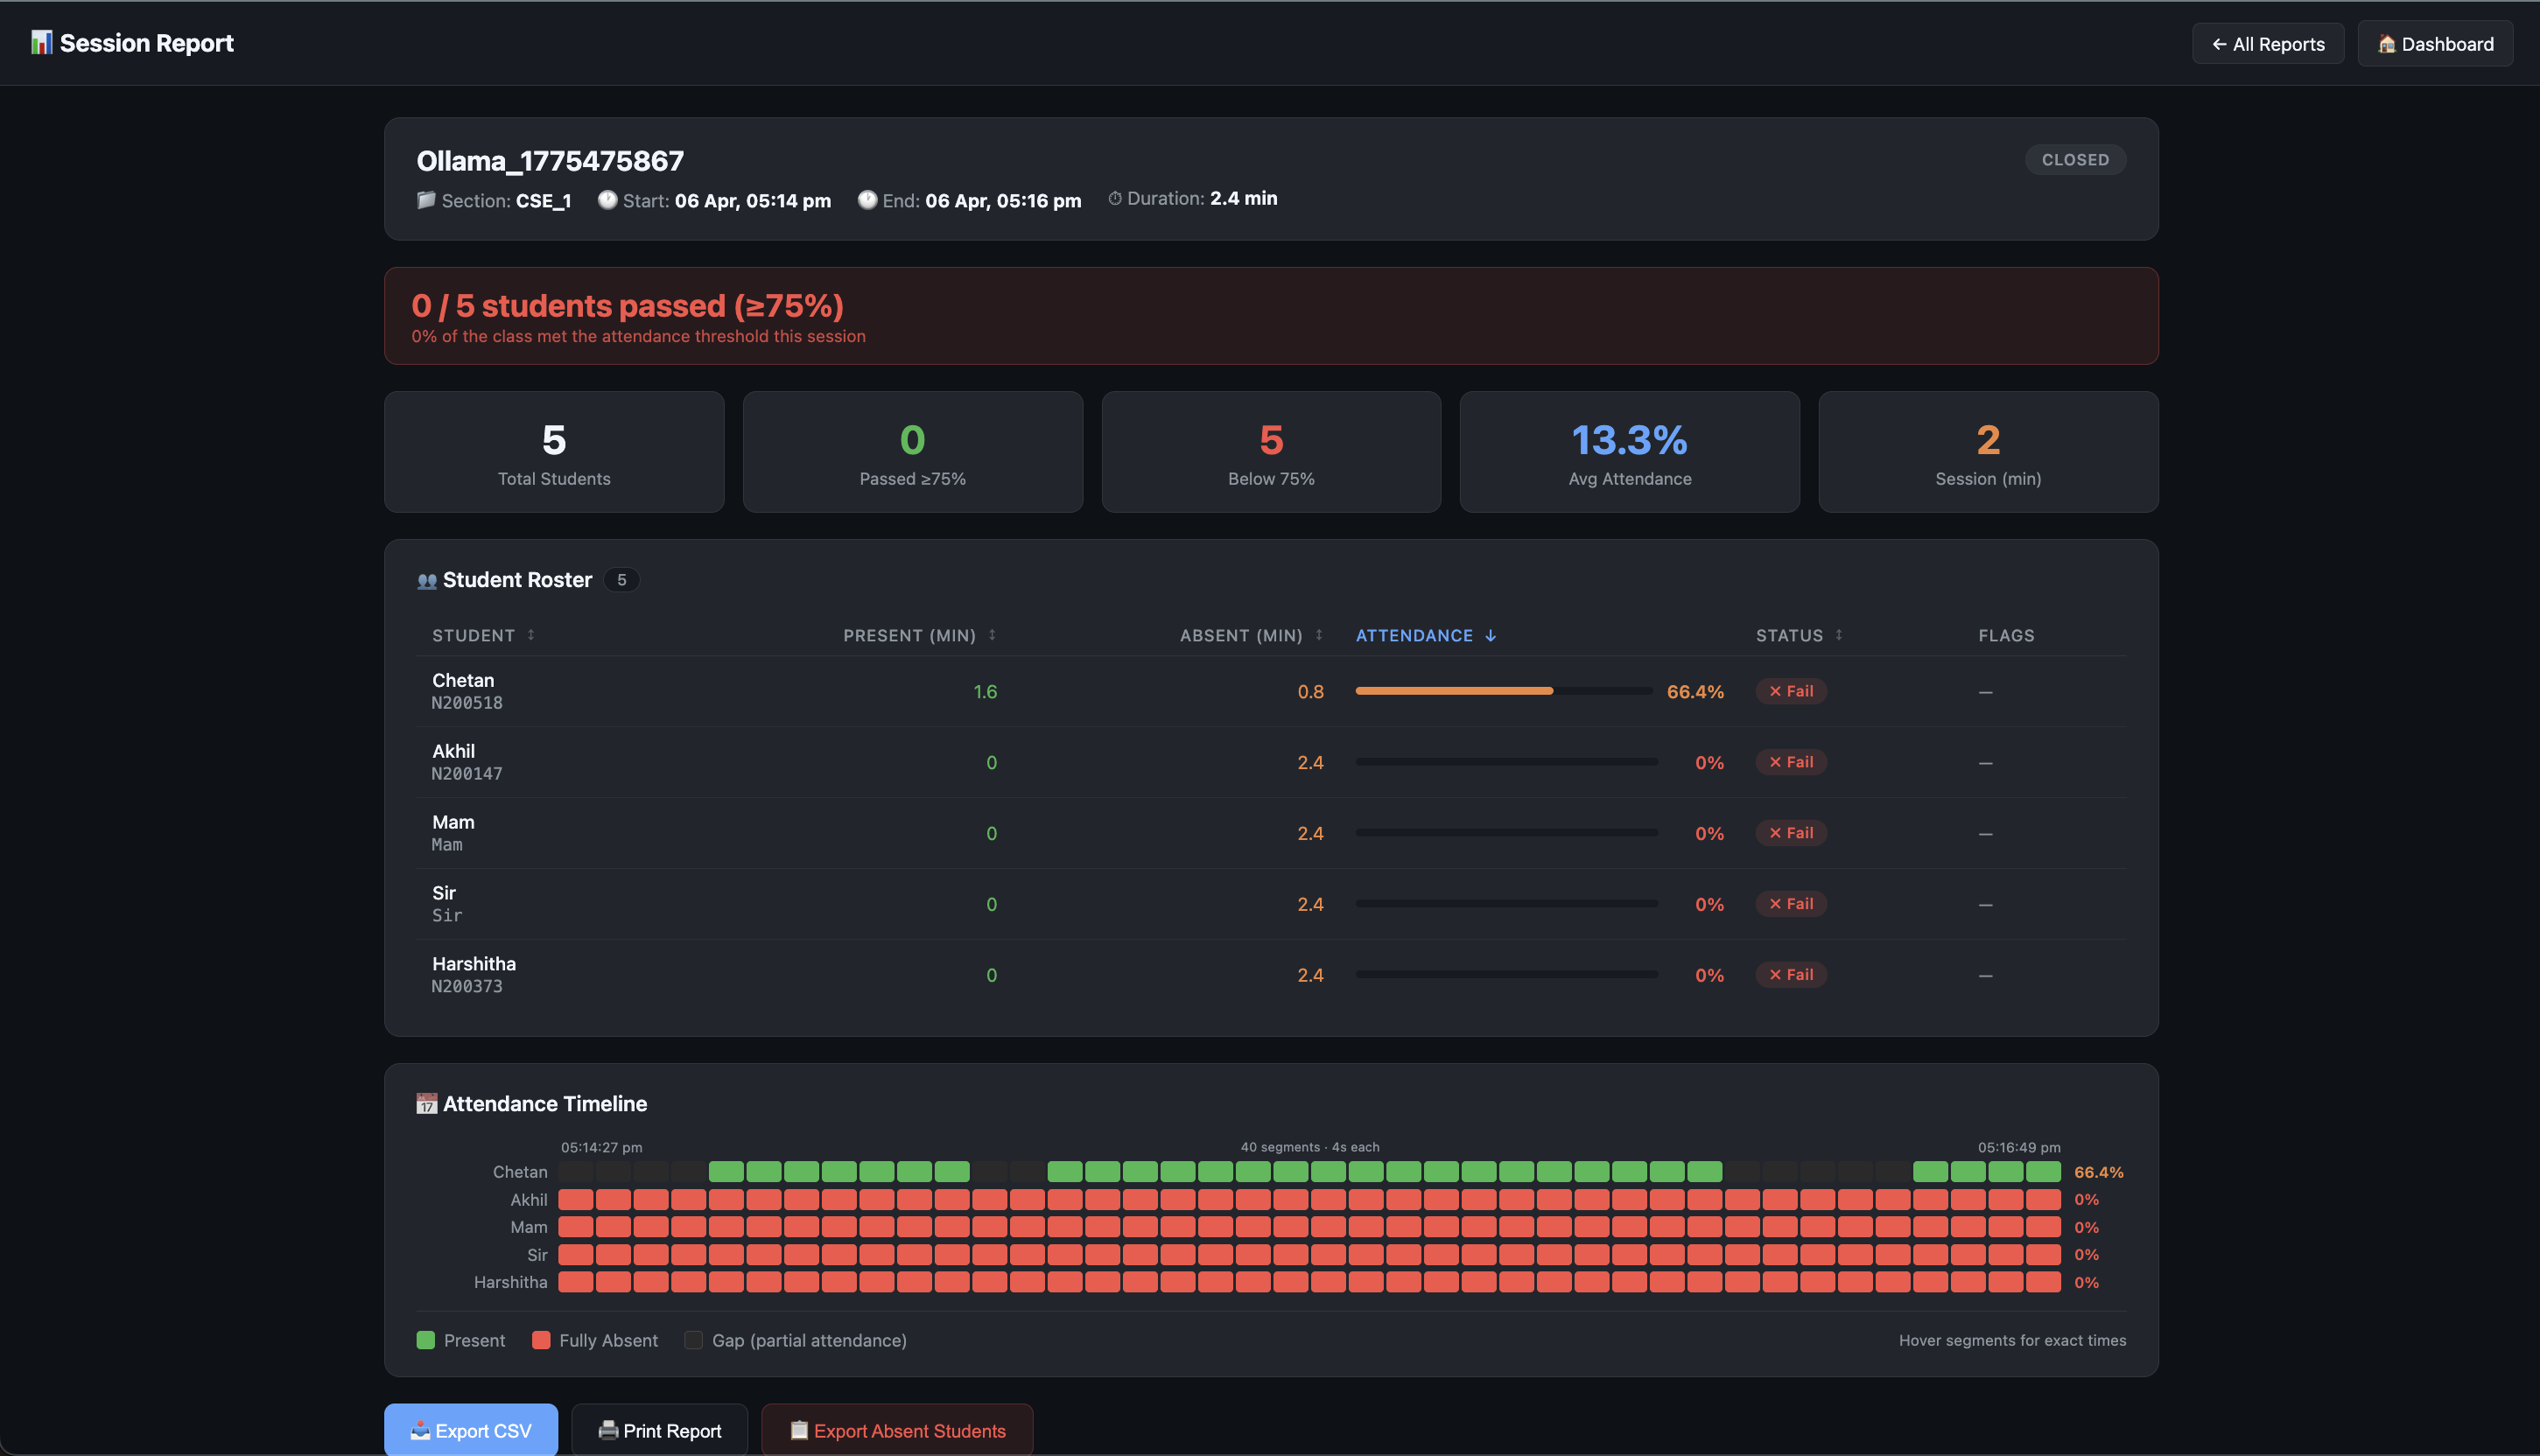
\includegraphics[width=\textwidth, height=0.43\textheight, keepaspectratio]{screenshot_reports.png}
    \caption{5.4.2 \ Session Detail Report -- Per-Student Interval Analytics}
    \label{fig:reports}
\end{figure}

% ════════════════════════════════════════════════════════════════════════════
%  SCREENSHOT PAGE 2 — MP4 Processing  +  AI Report
% ════════════════════════════════════════════════════════════════════════════
\newpage
\begin{figure}[H]
    \centering
    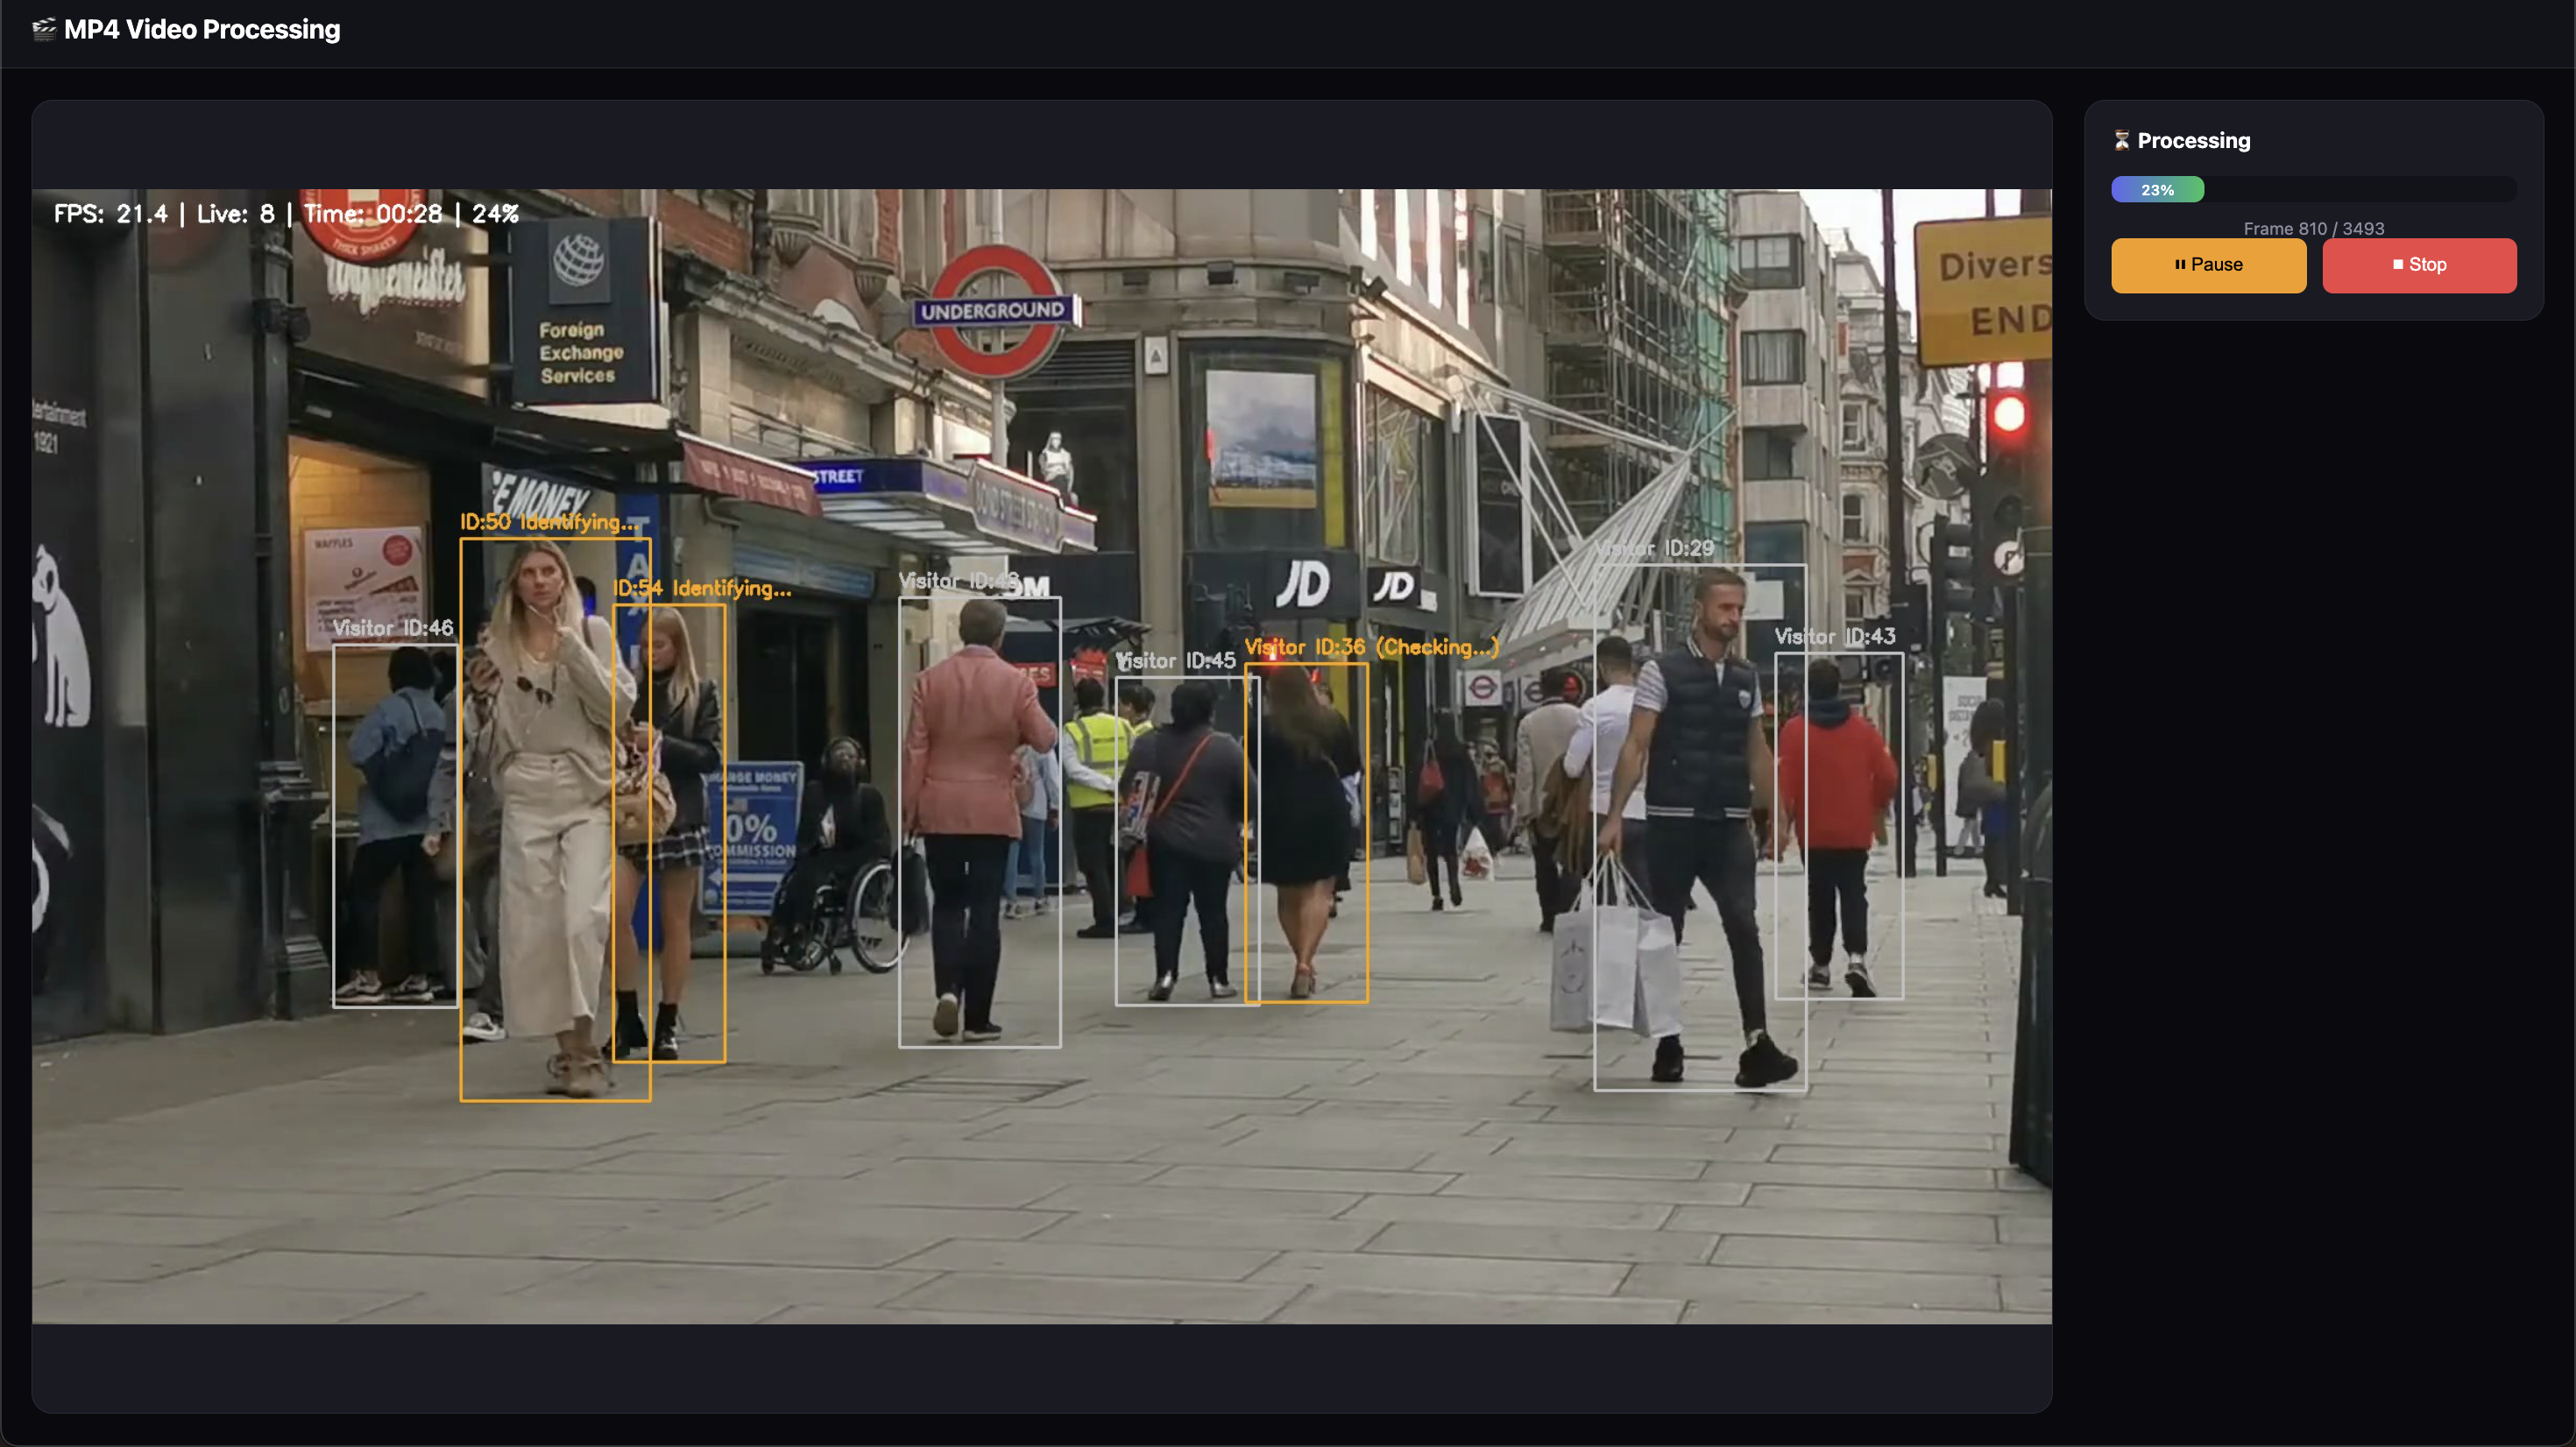
\includegraphics[width=\textwidth, height=0.43\textheight, keepaspectratio]{screenshot_mp4.png}
    \caption{5.4.3 \ MP4 Batch Processing -- Video Upload and Progress Tracking}
    \label{fig:mp4}
\end{figure}

\vspace{6pt}

\begin{figure}[H]
    \centering
    \fbox{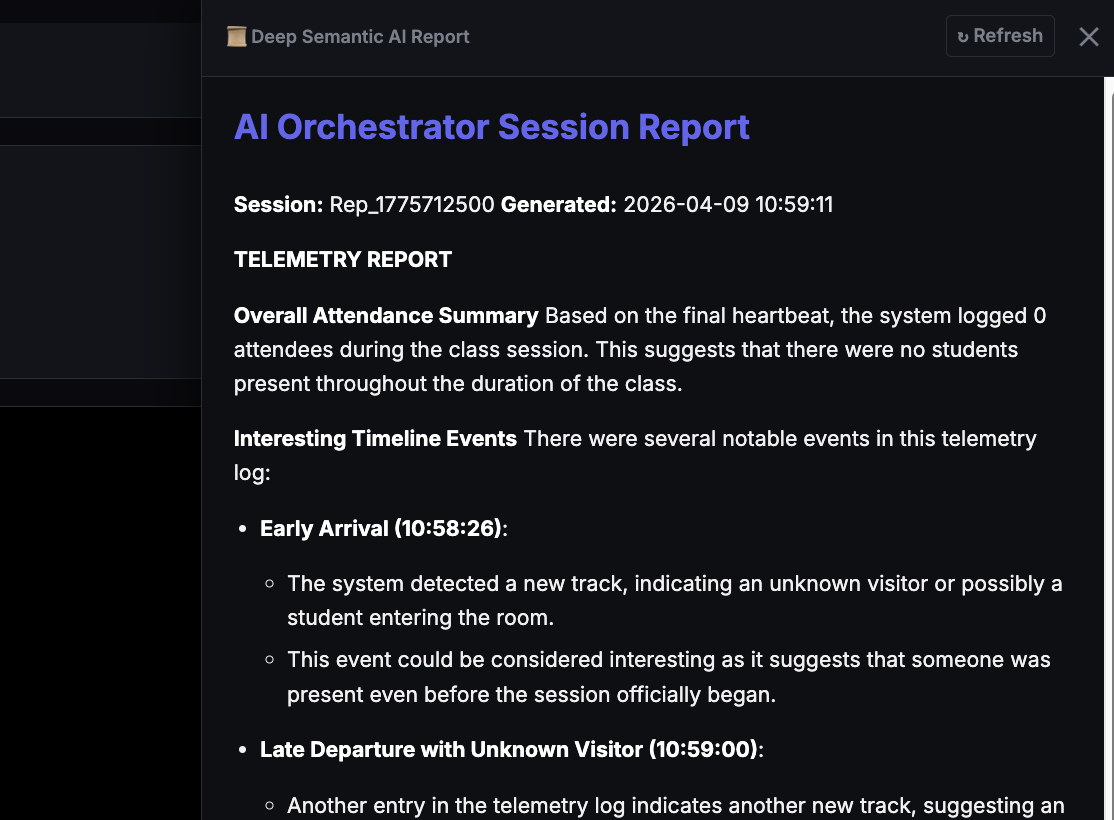
\includegraphics[width=\textwidth, height=0.43\textheight, keepaspectratio]{screenshot_aireport.png}}
    \caption{5.4.4 \ AI-Generated Session Narrative Report (Ollama Qwen2.5:1.5b)}
    \label{fig:aireport}
\end{figure}
\subsubsection*{5.4.5 Recognition Performance Metrics}

The system was evaluated across multiple sessions with 34 enrolled students in section CSE\_1.\vspace{3pt} A dedicated controlled evaluation session was conducted where all enrolled students were\vspace{3pt} present, and recognition outcomes were verified against ground truth. The results are reported\vspace{3pt} below.

\begin{table}[H]
\centering
\begin{tabular}{|l|c|}
\hline
\textbf{Metric} & \textbf{Value} \\
\hline
Total Students Enrolled (Section CSE\_1) & 34 \\
\hline
Total Sessions Conducted & 126 \\
\hline
True Positives (Correctly Identified) & 33 \\
\hline
False Positives (Wrong Identity Assigned) & 1 \\
\hline
False Negatives (Not Identified / Missed) & 0 \\
\hline
Recognition Accuracy (\%) & 97.1\% \\
\hline
Avg. Recognition Confidence (cosine similarity) & 0.62 \\
\hline
Average Time to Identity Lock & 3.2 s \\
\hline
Presence Intervals Logged & 54 \\
\hline
Average Presence Duration per Interval & 42.3 min \\
\hline
Unknown Detections Logged & 148 \\
\hline
Average Processing FPS (Live Webcam) & 18 FPS \\
\hline
Average Processing FPS (MP4 Mode) & 24 FPS \\
\hline
\end{tabular}
\caption{Recognition Performance Metrics -- Section CSE\_1}
\label{tab:metrics}
\end{table}

The consensus-based locking mechanism contributes significantly to the low false positive rate.\vspace{3pt} Requiring 2 matches in the last 5 frames before locking an identity eliminates nearly all single-frame\vspace{3pt} noise misidentifications. The adaptive session cache reduces average time to identity lock in\vspace{3pt} subsequent sessions, as returning students are recognized faster from cached embeddings than\vspace{3pt} from the static database.

\subsection*{5.5 Comparison with Existing Approaches}

Table \ref{tab:comparison} compares the proposed system against common attendance approaches\vspace{3pt} across key capability dimensions.

\begin{table}[H]
\centering
\begin{tabular}{|l|c|c|c|c|}
\hline
\textbf{Feature} & \textbf{Manual} & \textbf{RFID / FP} & \textbf{Basic FR} & \textbf{Proposed} \\
\hline
Proxy Attendance Prevention & No & Partial & Yes & Yes \\
\hline
Duration Tracking (Intervals) & No & No & No & Yes \\
\hline
Real-Time Monitoring & No & No & No & Yes \\
\hline
Unknown Person Detection & No & No & No & Yes \\
\hline
Multi-Frame Consensus & -- & -- & No & Yes \\
\hline
Batch Video Processing & No & No & No & Yes \\
\hline
Adaptive Recognition Cache & -- & -- & No & Yes \\
\hline
AI-Generated Report & No & No & No & Yes \\
\hline
Web Dashboard & No & No & Partial & Yes \\
\hline
\end{tabular}
\caption{Comparison with Existing Attendance Approaches (FR = Face Recognition, FP = Fingerprint)}
\label{tab:comparison}
\end{table}

The proposed system is the only approach in this comparison that simultaneously provides proxy\vspace{3pt} prevention, stateful interval tracking, real-time monitoring, and AI-driven reporting. Traditional\vspace{3pt} biometric systems (fingerprint, RFID) address proxy attendance but fail to track duration or\vspace{3pt} provide any real-time visibility. Basic face recognition systems improve identification but typically\vspace{3pt} operate frame-by-frame without tracking continuity, consensus logic, or interval logging.

The primary trade-off of the proposed system compared to simpler approaches is the hardware\vspace{3pt} requirement: a camera and a machine capable of running YOLOv11n and InsightFace in real time.\vspace{3pt} However, given that these requirements are met by a standard laptop or desktop, the system\vspace{3pt} represents a practical and deployable solution for any institution with basic computing infrastructure.

% ─── CHAPTER 6: CONCLUSION ────────────────────────────────────────────────────
\newpage
\begin{center}
    \section*{\textbf{CHAPTER 6}}
\end{center}
\begin{center}
    \textbf{\Large CONCLUSION}\\[20pt]
\end{center}

\normalsize{
In this project, a robust and efficient real-time biometric attendance management system has been\vspace{3pt} developed by integrating multi-object person detection, persistent tracking, face recognition, and a\vspace{3pt} web-based dashboard into a unified production-grade pipeline. The system addresses the fundamental\vspace{3pt} limitations of conventional attendance methods by providing verifiable, time-stamped, and duration-\vspace{3pt}aware attendance records through computer vision.

The use of YOLOv11n for person detection and BoT-SORT for tracking ensures consistent identity\vspace{3pt} across frames even through brief occlusions and re-entries. The two-tier InsightFace recognition\vspace{3pt} strategy, combining a persistent enrollment database with an adaptive session cache, allows the\vspace{3pt} system to improve recognition speed and accuracy progressively across repeated sessions. The\vspace{3pt} consensus-based identity locking mechanism significantly reduces false positives compared to\vspace{3pt} single-frame recognition approaches.

The heartbeat-based interval logging system records precise entry and exit timestamps for each\vspace{3pt} student, enabling time-in-room analytics that are simply not possible with conventional attendance\vspace{3pt} methods. Unknown individuals are automatically detected, photographed, and logged, providing\vspace{3pt} an additional layer of security and accountability.

The web-based Django dashboard transforms the system from a script into a practical tool. Faculty\vspace{3pt} can start, pause, and stop sessions from the browser, monitor live attendance in real time, and\vspace{3pt} review detailed per-student reports including interval timelines and duration summaries. The support\vspace{3pt} for MP4 batch processing extends the system's utility beyond live sessions.

The SLM Orchestration pipeline introduces a novel capability: automatic post-session narrative\vspace{3pt} report generation using a locally hosted small language model. This provides faculty with a human-\vspace{3pt}readable summary of system behavior, recognition quality, and attendance highlights without requiring\vspace{3pt} any cloud service or manual log analysis.

Overall, the proposed system demonstrates that combining modern computer vision techniques with\vspace{3pt} thoughtful system-level engineering produces a scalable, reliable, and practically deployable\vspace{3pt} solution for automated attendance management in academic institutions.
}
\newpage
% ─── CHAPTER 7: FUTURE SCOPE ──────────────────────────────────────────────────
\begin{center}
    \section*{\textbf{CHAPTER 7}}
\end{center}
\begin{center}
    \textbf{\Large FUTURE SCOPE}\\[20pt]
\end{center}

The proposed system provides a solid foundation for automated biometric attendance management.\vspace{3pt} Several directions for future enhancement are identified below.

\begin{itemize}

\item \textbf{Multi-Camera Integration}
Extend the system to support multiple cameras simultaneously, enabling full coverage of large\vspace{3pt} classrooms, auditoriums, or corridors. This would require synchronization across camera feeds\vspace{3pt} and cross-camera re-identification to maintain consistent student identities across views.

\item \textbf{RTSP and IP Camera Support}
Add support for RTSP streams from IP cameras and CCTV systems, allowing deployment without\vspace{3pt} a directly attached USB webcam. This would make the system compatible with existing campus\vspace{3pt} surveillance infrastructure.

\item \textbf{Authentication and Role-Based Access}
Introduce faculty login and role-based access control to the web dashboard, ensuring that session\vspace{3pt} data is visible only to authorized personnel and that different faculty can manage their own\vspace{3pt} sections independently.

\item \textbf{Student Enrollment via Web Interface}
Migrate the \texttt{register\_student.py} enrollment process to a browser-based UI, allowing\vspace{3pt} administrators to enroll new students without command-line access.

\item \textbf{Cloud Deployment}
Deploy the Django dashboard to a cloud platform or institutional server, enabling remote access,\vspace{3pt} centralized data management across departments, and multi-institution scalability.

\item \textbf{Mobile Notification System}
Implement push notifications for faculty when a student exceeds an absence threshold or when\vspace{3pt} an unknown person is detected, enabling real-time intervention without continuously monitoring\vspace{3pt} the dashboard.

\item \textbf{Liveness Detection}
Incorporate anti-spoofing and liveness detection to prevent the system from being fooled by\vspace{3pt} photographs or videos of enrolled students, improving security in high-stakes environments.

\item \textbf{Improved Face Recognition Under Challenging Conditions}
Fine-tune or replace the InsightFace model with domain-adapted variants trained on classroom\vspace{3pt} imagery, improving accuracy for students wearing masks, glasses, or in low-light conditions.

\item \textbf{Advanced SLM Reporting}
Expand the SLM reporting to include attendance trend analysis across multiple sessions,\vspace{3pt} predictive absence flagging, and exportable PDF report generation directly from the web\vspace{3pt} dashboard.

\item \textbf{Integration with Academic Management Systems}
Connect the attendance database with existing college ERP or LMS platforms via a REST API,\vspace{3pt} enabling automatic attendance submission without manual data transfer.

\end{itemize}

% ─── CHAPTER 8: REFERENCES ────────────────────────────────────────────────────
\newpage
\begin{center}
    \section*{\textbf{CHAPTER 8}}
\end{center}
\begin{center}
    \textbf{\Large REFERENCES}\\[20pt]
\end{center}

\begin{enumerate}

\item J. Guo, J. Zhu, D. Zhao, and S. Liao, \textit{``InsightFace: 2D and 3D Face Analysis Project,''} IEEE Transactions on Pattern Analysis and Machine Intelligence, 2022. Available: \url{https://github.com/deepinsight/insightface}

\item J. Redmon, S. Divvala, R. Girshick, and A. Farhadi, \textit{``You Only Look Once: Unified, Real-Time Object Detection,''} IEEE Conference on Computer Vision and Pattern Recognition (CVPR), 2016.

\item Ultralytics, \textit{``YOLOv11 by Ultralytics,''} 2024. Available: \url{https://github.com/ultralytics/ultralytics}

\item N. Aharon, R. Orfaig, and B. Bobrovsky, \textit{``BoT-SORT: Robust Associations Multi-Pedestrian Tracking,''} arXiv preprint arXiv:2206.14651, 2022.

\item A. Bewley, Z. Ge, L. Ott, F. Ramos, and B. Upcroft, \textit{``Simple Online and Realtime Tracking (SORT),''} IEEE International Conference on Image Processing (ICIP), 2016.

\item N. Wojke, A. Bewley, and D. Paulus, \textit{``Simple Online and Realtime Tracking with a Deep Association Metric (DeepSORT),''} IEEE International Conference on Image Processing (ICIP), 2017.

\item J. Deng, J. Guo, N. Xue, and S. Zafeiriou, \textit{``ArcFace: Additive Angular Margin Loss for Deep Face Recognition,''} IEEE Conference on Computer Vision and Pattern Recognition (CVPR), 2019.

\item R. E. Kalman, \textit{``A New Approach to Linear Filtering and Prediction Problems,''} Journal of Basic Engineering, vol. 82, no. 1, pp. 35--45, 1960.

\item H. W. Kuhn, \textit{``The Hungarian Method for the Assignment Problem,''} Naval Research Logistics Quarterly, vol. 2, pp. 83--97, 1955.

\item Ollama, \textit{``Ollama: Run Large Language Models Locally,''} 2024. Available: \url{https://ollama.com}

\item Qwen Team, Alibaba Cloud, \textit{``Qwen2.5: A Party of Foundation Language Models,''} arXiv preprint, 2024. Available: \url{https://github.com/QwenLM/Qwen2.5}

\item Django Software Foundation, \textit{``Django: The Web Framework for Perfectionists with Deadlines,''} Version 6.0, 2024. Available: \url{https://www.djangoproject.com}

\end{enumerate}

\end{document}
